\documentclass[12pt,a4paper,twoside,openright]{book}
\usepackage[top=0.9in,bottom=0.9in,inner=1.3in,outer=0.9in]{geometry}
\usepackage{fontspec}
\setmainfont{Times New Roman}
\usepackage{setspace}
\singlespacing
\usepackage{graphicx}
\usepackage{rotating}
\usepackage{caption}
\usepackage{booktabs}
\usepackage{longtable}
\usepackage{array}
\usepackage{titlesec}
\usepackage{fancyhdr}
\usepackage[hidelinks]{hyperref}
\usepackage{tocloft}
\usepackage{seqsplit}
\emergencystretch=2.5em
\renewcommand{\bibname}{References}
\setcounter{tocdepth}{2}
\setcounter{secnumdepth}{3}
\captionsetup{font=small,labelsep=period}

\titleformat{\chapter}[display]
  {\normalfont\fontsize{20}{24}\selectfont\bfseries\vspace*{\fill}}
  {\centering\MakeUppercase\chaptername~\thechapter}
  {1em}
  {\centering\MakeUppercase}
\titlespacing*{\chapter}{0pt}{30pt}{50pt}

\pagestyle{fancy}
\fancyhf{}
\fancyfoot[LE,RO]{\thepage}
\renewcommand{\headrulewidth}{0pt}
\renewcommand{\footrulewidth}{0pt}
\fancypagestyle{plain}{%
  \fancyhf{}%
  \renewcommand{\headrulewidth}{0pt}%
  \renewcommand{\footrulewidth}{0pt}%
}

\makeatletter
\renewcommand{\cleardoublepage}{%
  \clearpage
  \if@twoside
    \ifodd\c@page\else
      \thispagestyle{empty}\hbox{}\newpage
      \if@twocolumn\hbox{}\newpage\fi
    \fi
  \fi}
\makeatother

\begin{document}

\frontmatter
\tableofcontents
\cleardoublepage
\listoffigures
\cleardoublepage
\listoftables
\thispagestyle{fancy}

\chapter*{Abstract}
\addcontentsline{toc}{chapter}{Abstract}

Educational institutions that serve large numbers of students manage a
fragmented workflow: syllabi must be structured manually, printed study
material must be converted to machine-readable text, question sets are
authored by hand, and examinations are assembled, scheduled, attempted, and
evaluated across separate systems. This project designs and implements
CatLium EduTech, a multi-tenant Software-as-a-Service platform that automates
this complete lifecycle from raw syllabus and study material to a delivered,
evaluated examination.

The platform is implemented as a modular monolith: a single NestJS
(TypeScript) API that hosts the business domains, an independent Python
stack that provides an OCR service and asynchronous RabbitMQ-based workers
for AI-driven and material-processing workloads, and a Next.js web
application used by institute administrators, teachers, and students. Every
data access is scoped to an institute through a membership-based tenancy
model, with cookie-based session authentication, CSRF protection, and role
based authorization. Content flows through a deterministic pipeline: syllabus
documents are proposed as chapter--topic hierarchies by an AI assistant
under teacher review; PDF and image materials are converted to page-accurate
text by an OCR service; a Material Intelligence engine cleans, structures,
and segments the extracted text and maps it to syllabus entities; and a
question bank feeds paper patterns, question papers, and assessments that
students attempt with server-side deadline enforcement and deterministic
evaluation of objective question types. Study content (notes, summaries,
flashcards, and concepts) is generated by AI workers through an internal
OpenAI-compatible gateway, with schema validation on both worker and API
boundaries.

The system is validated by 188 API unit tests, 118 Python tests across the
OCR and worker services, 15 web tests, and end-to-end harnesses that
exercise the live stack through its public gateway. The report documents the
analysis, design, implementation, testing, and results of the completed
system, and clearly separates implemented scope from deferred future work.
\chapter*{List of Abbreviations}
\addcontentsline{toc}{chapter}{List of Abbreviations}

\begin{longtable}{@{}p{3.2cm}p{\dimexpr\textwidth-3.2cm-12pt\relax}@{}}
\toprule
\textbf{Abbreviation} & \textbf{Full form} \\
\midrule
\endhead
AI & Artificial Intelligence \\
API & Application Programming Interface \\
B.Sc. & Bachelor of Science \\
CSRF & Cross-Site Request Forgery \\
DOCX & Microsoft Word Open XML document format \\
E2E & End-to-end \\
ERD & Entity--Relationship Diagram \\
HTTP & Hypertext Transfer Protocol \\
JSON & JavaScript Object Notation \\
JSONB & Binary JSON (PostgreSQL) \\
JWT & JSON Web Token \\
LLM & Large Language Model \\
LMS & Learning Management System \\
OCR & Optical Character Recognition \\
PDF & Portable Document Format \\
RBAC & Role-Based Access Control \\
SaaS & Software-as-a-Service \\
SQL & Structured Query Language \\
UI & User Interface \\
XLSX & Microsoft Excel Open XML spreadsheet format \\
ZOD & TypeScript-first schema validation library \\
\bottomrule
\end{longtable}

\mainmatter
\chapter{Introduction}
\label{ch:introduction}

\section{Background and Motivation}

Colleges continuously invest in preparation and assessment materials:
syllabi, textbooks, notes, practice questions, and examinations. In most
institutions these assets are created and managed with generic office tools and
file storage. The consequences are well known: teaching material is duplicated
or lost, syllabus meaning has to be manually re-derived for every subject,
question banks accumulate without validation of correctness or alignment with
exam patterns, and assessments are distributed and evaluated manually, so
students receive little or no structured feedback.

The project team built a platform that addresses these problems as \textbf{a
multi-tenant, role- and permission-controlled web application} for educational
institutes. A single deployment serves many institutes on one shared codebase,
yet keeps every institute's data isolated and inaccessible to the others. The
platform makes the preparation-and-assessment workflow structured: uploaded
materials are OCR-processed into reusable text, syllabus documents are analysed
into confirmed curriculum structures, study content is generated
semi-automatically, question banks are built against explicit paper patterns,
and assessments are scheduled, taken, and evaluated server-side.

\section{Problem Statement}

\noindent The problem addressed by this project is stated as follows:

\emph{Educational institutes require a single, tenant-isolated platform that (i)
converts unstructured teaching material (scanned PDFs, images, documents) into
structured, searchable content through OCR and AI-assisted processing; (ii)
turns syllabus documents into confirmed academic structures; (iii) builds
curated question banks and examination assets from declarative paper patterns;
(iv) runs scheduled assessments with automatic server-side evaluation and
meaningful analytics; (v) offers ungraded practice for students; and (vi)
exports all assets in standard, print-ready formats --- all while restricting
every operation to the acting user's role, permissions, and academic scope.}

\section{Objectives}

\noindent The specific objectives of the implementation are:

\begin{enumerate}
  \item \textbf{Tenancy and identity:} model institutes, memberships, roles, and
  users, and isolate data per tenant.
  \item \textbf{Academic structure:} model years, classes, divisions, subjects,
  class--subject offerings, and teacher/student assignments, and derive each
  actor's academic scope from that structure.
  \item \textbf{Materials and OCR:} upload PDF, image, and document materials
  with chunked upload, process them through a distributed OCR pipeline with
  embedded-text-first extraction and PaddleOCR fallback, and expose per-page
  corrections.
  \item \textbf{Syllabus intelligence:} analyse syllabus documents into a
  confirmed global curriculum with topics, units, objectives, and learning
  outcomes.
  \item \textbf{Aided content creation:} generate notes, flashcards, Cornell
  notes, summaries, and important-concepts content from eligible source
  materials through an async AI generation pipeline, with provenance.
  \item \textbf{Question assets:} establish a data-driven question-type system
  and a question bank with generation, approval states, ranking, and difficulty
  distribution; build paper patterns and question papers from blueprints.
  \item \textbf{Examination:} author assessments from blueprints, publish and
  activate them on schedules, record attempts with immutable question
  snapshots, evaluate objective answers server-side, and produce aggregate
  analytics.
  \item \textbf{Practice:} provide flashcard and question practice modes with
  instant per-item feedback and no grading.
  \item \textbf{Export:} generate print-ready PDF, DOCX, and XLSX outputs for
  content, questions, papers, and results.
  \item \textbf{Security and architecture:} enforce tenant isolation at the
  data layer, security decisions from an explicit permission catalogue, and
  strictly internal compute for OCR and AI via a provider gateway.
\end{enumerate}

\section{Scope}

The implemented system covers the full lifecycle described above. It does not
implement online-answer-sheet (FORM), OMR-scanning, or on-screen-marking
checking features, automated grading of subjective (essay-type) answers, or
per-attempt N-of-M mechanics; these are identified as deferred future work in
Chapter~\ref{ch:conclusion}.

\section{Organisation of the Report}

\noindent Chapter~\ref{ch:literature-review} reviews related systems and
technologies. Chapter~\ref{ch:requirements} presents the requirements
analysis. Chapter~\ref{ch:methodology} describes the development methodology and
the project timeline. Chapter~\ref{ch:architecture} describes the system
architecture and Chapter~\ref{ch:database-design} the database design.
Chapter~\ref{ch:security} details the security and authorization architecture,
and Chapter~\ref{ch:features} explains the core features and their workflows.
Chapter~\ref{ch:implementation} covers implementation details,
Chapter~\ref{ch:testing} the testing and validation strategy, and
Chapter~\ref{ch:results} the results and discussion.
Chapter~\ref{ch:conclusion} concludes the report and lists future scope.
\chapter{Literature Review and Existing Systems}
\label{ch:literature-review}

\begin{center}
\textit{This chapter reviews existing systems and technologies relevant to
the platform --- learning management systems, optical character recognition,
large language models in education, multi-tenancy, authorization models, and
asynchronous processing patterns --- and identifies the gap that the project
addresses.}
\end{center}

\vspace*{\fill}
\clearpage
\section{Existing Educational Platforms}

Learning management systems (LMS) such as Moodle~\cite{moodle}, Google
Classroom~\cite{gclassroom}, and Canvas~\cite{canvas} provide course delivery,
assignments, and basic content organization to whole institutions. They are
strong at the operational layer --- announcing courses, distributing
assignments, and tracking participants --- but expose limited support for the
specific preparation-and-assessment workflow this project targets: turning
uploaded textbook chapters and previous-year papers into structured content,
a structured question bank aligned to an exam blueprint, and scheduled
server-evaluated assessments. Such platforms do not typically perform OCR of
arbitrary educational documents, nor do they generate study content and
examination assets with an AI pipeline and provenance for every produced
artifact.

Commercial and open-source tools exist for individual pieces of the workflow.
OCR engines such as Tesseract and PaddleOCR extract text from scanned pages;
document libraries such as PyMuPDF give programmatic access to PDF text and
page rasterisation; AI content tools produce text on demand; quiz systems
evaluate objective questions. The gap addressed here is a single
tenant-isolated system that \emph{integrates} these pieces with an explicit
authorization model, so that a college gets one coherent asset pipeline from
``upload'' to ``evaluate''.

\section{Optical Character Recognition}

Tesseract is a long-established open-source OCR engine with excellent
support for structured Latin-script documents~\cite{tesseract}. For
handwritten and complex scripts, deep-learning OCR models are more robust.
The PaddleOCR line of models (PP-OCR)~\cite{ppocr} provides lightweight,
practical, multilingual OCR pipelines from the PaddlePaddle ecosystem and is
widely used for real-world degradation (noise, watermarks, low contrast).
Document payloads almost always live inside PDF files, which may contain an
embedded digital text layer (born-digital PDFs) or be pure scans. PyMuPDF
gives safe, dependency-light access to both: it extracts embedded text per
page and rasterises pages to images for OCR fallback~\cite{pymupdf}.

The design decision of this project is \emph{embedded-text-first, OCR-fallback
per page}: a page whose embedded text has a usable length (at least five
characters) is accepted directly, and only otherwise is it rasterised and
passed to PaddleOCR. This reduces OCR load, preserves born-digital fidelity,
and reserves compute for genuinely scanned material. OCR output is then
normalised by a deterministic character pass, and the resulting text is stored
on the material row so it can feed AI generation and text-based reuse without
re-running vision models.

\section{Large Language Models in Education}

Transformer-based language models~\cite{vaswani2017} have made
instruction-following generation practical for educational content. A
retrieval-augmented pattern --- supply selected source material as context,
then generate the desired artifact (notes, flashcards, summaries, questions)
--- is the dominant integration shape for factual document-derived content
because it grounds the output in the source document and makes the 
\emph{source of truth} explicit~\cite{lewis2020rag}. This project follows that
pattern: the AI worker assembles a bounded context budget from READY source
materials, calls the model through an internal gateway, validates each
response against strict schemas for the requested artifact, and stores
generated items with provenance linking them to the exact source revisions
used. Responses that fail schema validation or transient transport are
retried with backoff up to a maximum number of attempts; terminal errors
settle the associated job as failed rather than leaving it in a running state.

\section{Multi-tenant Architecture}

Multi-tenancy spans a spectrum from isolated deployments (one stack per
tenant) through shared-database models (each tenant's rows prefixed or
separated) with varied data-security trade-offs. The implementation chooses a
shared-schema, tenant-scoped model: one PostgreSQL database whose tables carry
an \texttt{institute\_id}, and every query that touches user data is filtered
by the resolved active institute. Tenant resolution comes from an explicit
header chosen by the client on each request, validated by a guard that checks
a live, active membership. This yields low operational cost and strong
consistency, and it is defensible because the enforcement is at the query
layer rather than the presentation layer.

\section{Authorization Models}

Authorization is classically organised as role-based access control (RBAC),
in which roles bundle rights, or attribute- and policy-based models that
evaluate rules on each request. Pure RBAC is simple but coarse: a ``teacher''
role grants the same rights over every class the teacher teaches, which leaks
access across cohorts. Permission-based models refine RBAC by evaluating the
\emph{permission key} (e.g. \texttt{questions.update}) and, additionally, by
restricting \emph{where} that permission may operate (the academic scope).
Libraries such as CASL provide attribute-based policy evaluation for such
models~\cite{casl}, but this project implements its own compact engine ---- a
single typed permission catalogue with a fixed \texttt{resource.action}
vocabulary, default-deny, a \texttt{manage}-implies action rule, and no
wildcards ---- deliberately avoiding a dependency for a decision that is at
its core a few deterministic predicates. Roles become permission bundles: the
built-in \texttt{INSTITUTE\_ADMIN}, \texttt{TEACHER}, and \texttt{STUDENT}
roles, plus an institution-level \texttt{SUPER\_ADMIN} platform plane that is
kept disjoint from institute membership.

\section{Asynchronous Processing Patterns}

Long-running operation must not block an API request. The classic pattern is a
message broker with durable queues and worker consumers: the API writes a
job row, publishes a message, returns \texttt{202 Accepted} with the job id,
and a worker consumes the message, does the work, and settles the job. This
project uses RabbitMQ~\cite{rabbitmq} with two queues --- one for material
processing and one for AI generation with bounded concurrency. A variant for
the OCR pipeline is a \emph{coordinator-owned} design: the API itself owns the
OCR chunk registry, leases chunks to registered OCR workers by claim, and
reclaims idle or expired leases, because OCR compute nodes are expected to be
flaky, heterogeneous, and occasionally offline. This combination (queue for
message-based work, coordinator for lease-based work) preserves the
API-never-blocks guarantee while tolerating worker loss.

\section{Security Baseline}

Web authentication on this platform follows the OWASP cookie-session
recommendations~\cite{owaspcsfr, owaspsession}: short-lived httpOnly access
cookies, refresh tokens kept server-side as hashes, double-submit CSRF
protection on all state-changing requests, origin checks on credential
submission, and throttling. JWTs~\cite{rfc7519} are used only as
transport-format access tokens and carry no permissions; authorization is
re-evaluated from the current database state per request. Password hashing
uses bcrypt~\cite{bcrypt}, session hashes use SHA-256 per
FIPS~PUB~180-4~\cite{fips180}, and all internal service traffic is carried
over the private Docker network with shared or per-worker keys.

\section{Identified Gap}

Existing systems separately provide LMS features, OCR, AI generation, quiz
evaluation, or multi-tenancy. None of them combine, in one tenant-isolated
product, the end-to-end lifecycle of \emph{OCR-of-materials ---\,
AI-grounding ---\, syllabus structuring ---\, question-bank and paper-pattern
authoring ---\, scheduled server-evaluated assessments ---\, practice ---\,
print-ready export}, under an authorization model that restricts both the
\emph{actions} and the \emph{academic scope} of every actor. This project
targets exactly that gap; its contribution is architectural integration and a
security posture where tenant isolation is enforced by the enforcement layers
by default, not by incidental query shape.
\chapter{System Analysis and Requirements}
\label{ch:requirements}

\section{Analysis of the Existing Workflow}

\noindent Before design, the current workflow in a typical college was
analysed and the following recurring weaknesses identified:

\begin{itemize}
  \item \textbf{Fragmented material.} Course material exists as scattered
  PDFs and scans that are hard to search, reuse, or convert into other
  formats.
  \item \textbf{No syllabus structure.} Syllabus documents are read manually
  and translated into teaching plans repeatedly for each batch.
  \item \textbf{Uncontrolled question creation.} Questions are composed ad hoc
  without tracking origin, approval, or alignment to the examination pattern.
  \item \textbf{Manual assessment.} Distribution, collection, and evaluation
  are manual, giving students delayed and summary-only feedback.
  \item \textbf{No access discipline.} Generic shared logins mean no
  accountability and no restriction of what a user may do or where.
\end{itemize}

\section{Functional Requirements}

\noindent The functional requirements of the platform are grouped by area. Each
requirement is implemented and verified (see Chapter~\ref{ch:testing}).

\begin{center}
\small
\begin{longtable}{@{}p{1.6cm}p{12.4cm}@{}}
\toprule
\textbf{ID} & \textbf{Functional requirement} \\
\midrule
\endhead
FR-01 & Institute-scoped user login with short-lived access sessions and
refresh rotation. \\
FR-02 & Multiple institutes served from one deployment with strict data
isolation per institute. \\
FR-03 & Institute admin creates users (teachers, students), assigns roles, and
manages role permissions from an explicit catalogue. \\
FR-04 & Academic structure: academic years, classes, divisions, subjects,
class--subject offerings, teacher assignments, and student placements. \\
FR-05 & Upload teaching material (PDF, image, document, or text) with chunked
upload for large files. \\
FR-06 & Distributed OCR processing: embedded-text-first extraction with
per-page PaddleOCR fallback, chunk leasing, and retry; per-page text
corrections. \\
FR-07 & AI syllabus analysis producing a confirmed global curriculum (chapters,
topics, units, objectives, learning outcomes). \\
FR-08 & AI generation of study content (notes, flashcards, Cornell notes,
summaries, important concepts) from eligible sources with provenance. \\
FR-09 & Question types as data (global starters plus institute-custom types). \\
FR-10 & Question bank CRUD with approval workflow and difficulty/source
tracking. \\
FR-11 & AI question-bank generation in batches with pattern-coverage checks
(COVERED, AWAITING\_APPROVAL, INSUFFICIENT, GENERATING). \\
FR-12 & Paper patterns: manual authoring, text/material analysis, deterministic
validation, and approval-to-lock. \\
FR-13 & Question papers: selection from pattern, coverage checking, generation
of missing items, and conversion to assessments. \\
FR-14 & Assessments: authoring, pattern-based selection, publishing,
activation, and completion with schedule validation. \\
FR-15 & Student attempts: timed start with an immutable question snapshot,
per-answer saving, and idempotent submission with server-side evaluation. \\
FR-16 & Aggregate analytics: score distribution, per-question accuracy, and
topic/difficulty performance. \\
FR-17 & Ungraded practice: flashcard sessions and question sessions with
instant per-item feedback and no score. \\
FR-18 & Export to PDF, DOCX, and XLSX for content, question sets, papers,
patterns, and results. \\
FR-19 & Asynchronous job lifecycle with retry, cancel, and status polling. \\
FR-20 & Health checks for the API and OCR service. \\
\bottomrule
\end{longtable}
\end{center}

\section{Non-functional Requirements}

\begin{center}
\small
\begin{longtable}{@{}p{1.6cm}p{12.4cm}@{}}
\toprule
\textbf{ID} & \textbf{Non-functional requirement} \\
\midrule
\endhead
NFR-01 & \textbf{Security.} Cookie-based sessions with httpOnly attributes,
double-submit CSRF on state-changing requests, origin check on login, and
throttling on authentication endpoints. \\
NFR-02 & \textbf{Tenant isolation.} Every query touching user data is scoped
by the active institute; cross-tenant access must fail by default of the
enforcement layers. \\
NFR-03 & \textbf{Authorization.} Permission keys are DB-fresh per request with
default-deny and \texttt{manage} implication; academic scope restricts
permission reach. \\
NFR-04 & \textbf{Availability of the API.} The API never blocks on long
operations; heavy work happens in workers and returns \texttt{202 Accepted}. \\
NFR-05 & \textbf{Scalability of OCR and AI.} OCR compute is distributed and
lease-based; AI generation has bounded concurrency to protect the model
gateway. \\
NFR-06 & \textbf{Maintainability.} Monorepo with TypeScript packages shared
between web and API; typed shared contracts; strict typing in both TypeScript
and Python codebases. \\
NFR-07 & \textbf{Portability.} Everything runs from one Docker Compose file
with no service exposed on a host port in production. \\
NFR-08 & \textbf{Traceability.} Generated AI artifacts store provenance
(source type, source id, revisions) and are marked AI-generated. \\
\bottomrule
\end{longtable}
\end{center}

\section{User Roles}

\noindent The platform defines three built-in membership roles and one
disjoint platform role:

\begin{itemize}
  \item \textbf{Institute admin (\texttt{INSTITUTE\_ADMIN}):} full management
  of an institute's structure and content; holds \texttt{manage} across the
  institute permission catalogue and whole-institute academic scope.
  \item \textbf{Teacher (\texttt{TEACHER}):} creates and manages teaching
  material, content, syllabus, questions, patterns, question papers, and
  assessments within their assigned subjects; reads results and analytics.
  \item \textbf{Student (\texttt{STUDENT}):} reads content and materials within
  their placement scope, takes assessments (creating attempts), and uses
  practice sessions.
  \item \textbf{Platform admin (\texttt{SUPER\_ADMIN}):} operates on the
  platform plane (institutes, OCR worker registry) through platform-domain
  permissions, disjoint from institute membership.
\end{itemize}

\section{Constraints and Assumptions}

\begin{itemize}
  \item \textbf{Data.} PostgreSQL is the only primary database; MongoDB and
  SQLite are not permitted.
  \item \textbf{AI access.} AI calls must go through an internal provider
  gateway; no direct cloud AI SDK is called from application code.
  \item \textbf{Delegation.} Only OCR and asynchronous AI generation are
  permitted to move off the request thread; the API remains a single
  modular monolith.
  \item \textbf{Provisioning.} Users are provisioned by the institute, not by
  public self-registration.
  \item \textbf{Text evaluation.} Only objective question formats are
  auto-graded; subjective answers are recorded but not graded.
  \item \textbf{Fonts and documents.} Exported assets must be deterministic and
  printable; PDF generation is browser-based.
\end{itemize}

\section{Environment of Use}

\noindent The system runs as a Docker Compose stack. Its runtime environment
comprises a PostgreSQL~17 database, RabbitMQ~3 message broker, Node.js~20
(TypeScript) API and web services, a Python~3.12 OCR service, Python workers, an
internal AI gateway, an nginx reverse proxy, and a Cloudflare Tunnel for the
only public ingress. No internal service is published on a host port in
production.
\chapter{Development Methodology and Project Timeline}
\label{ch:methodology}

\section{Methodology}

The project follows an \textbf{iterative, incremental, checkpoint-driven}
development methodology. Work is organised as phases, each decomposed into
goals and tasks, and each meaningful unit of work ends in a validated,
documented, and committed checkpoint. The cycle used repeatedly throughout
development is:

\begin{center}
\small
\begin{tabular}{@{}c@{\qquad}c@{\qquad}c@{\qquad}c@{\qquad}c@{}}
Phase & $\rightarrow$ & Feature & $\rightarrow$ & Implementation \\
& $\rightarrow$ & Validation & $\rightarrow$ & Documentation \\
& $\rightarrow$ & Commit & $\rightarrow$ & Push \\
\end{tabular}
\end{center}

\noindent This style has two concrete consequences for the engineering process:

\begin{itemize}
  \item \textbf{Architecture decisions are recorded.} Seven architectural
  decisions (D1--D7) covering the permission model, role storage, the platform
  plane, academic structure, teacher/student assignments, resource scope, and
  session hardening were written down, decided, and then implemented in
  separate phases. A separate \textbf{documentation audit} (Phase~M) verified
  that the documents matched the code, rather than the reverse.
  \item \textbf{Validation is staged.} Schema changes are generated as
  Drizzle migrations, reviewed, and applied; TypeScript is type-checked; unit
  tests run on every change; database-backed integration suites run against
  PostgreSQL when available; and a human test-data (seeded demo) pass confirms
  user-observable behaviour before a phase is declared complete.
\end{itemize}

\noindent Scrum-like ceremonies are intentionally light: a single
product-oriented backlog (\texttt{docs/tasks.md}) holds the hierarchy, and the
project status file (\texttt{\seqsplit{docs/project-status.md}}) acts as the standing
checkpoint log so that work can resume across devices and sessions.

\section{Version Control and Continuity}

\noindent Work is committed to Git with conventional, scoped messages
(\texttt{feat(exams): publish to activate}) after each validated unit, and
pushed before interruptions (device switches, session ends). This makes the
repository itself the recovery protocol: any engineer can reconstruct the
state of the project from the tracker, status log, and Git history without
relying on conversation history.

\section{Project Timeline}

The project runs over Semester~V, from 1~July~2026 to 30~September~2026, in
seven planned phases. Table~\ref{tab:timeline} states the planned scope of each
phase and Figure~\ref{fig:gantt} renders the schedule as a Gantt chart.

\begin{table}[h]
\centering
\small
\begin{tabular}{@{}p{3.0cm}p{2.8cm}p{8.2cm}@{}}
\toprule
\textbf{Phase} & \textbf{Period (2026)} & \textbf{Planned scope} \\
\midrule
Analysis and planning & July 1--14 & Problem identification and requirement
analysis, study of academic guidelines, definition of scope and objectives. \\
System design & July 15--31 & System analysis, module decomposition,
architecture design (modular monolith), database schema design, technology
selection, project setup. \\
Core development & August 1--14 & Identity, tenancy, and authentication;
academic structure; material upload and the OCR processing pipeline. \\
Feature development & August 15--31 & AI-assisted syllabus structuring,
study-content generation, question bank, paper patterns, question papers, and
assessment authoring. \\
Examination and practice & September 1--14 & Scheduled assessments, student
attempts and evaluation, results and analytics, practice, export, and
interface hardening. \\
Testing and documentation & September 15--24 & Integration testing and
debugging, end-to-end validation, and project documentation. \\
Final review and submission & September 25--30 & Final review, correction, and
submission. \\
\bottomrule
\end{tabular}
\caption{Project timeline (Semester V, 2026).}
\label{tab:timeline}
\end{table}

\begin{figure}[h]
\centering
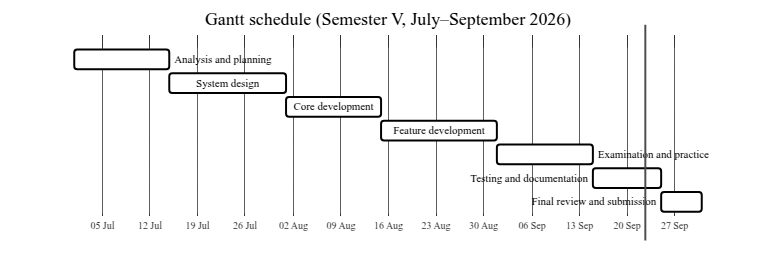
\includegraphics[width=\textwidth]{figures/gantt-chart.png}
\caption{Gantt chart of the seven project phases (July--September 2026).}
\label{fig:gantt}
\end{figure}

\section{Technologies Selected}

\noindent The technology stack, justified in detail in
Chapter~\ref{ch:implementation}, is summarised below: a TypeScript modular
monolith (NestJS) for the API; Next.js for the web client; PostgreSQL~17 with
Drizzle ORM as the single database; Redis for cache and RabbitMQ~3 for
messaging; a FastAPI OCR service and Python workers for heavy processing; a
provider-gateway integration for AI; Zod and Pydantic for schema validation at
the contract boundary; and Docker Compose plus a reverse proxy with a Cloudflare
Tunnel for deployment.
\chapter{System Architecture}
\label{ch:architecture}

\section{Architectural Style}

\noindent The system uses three cooperating kinds of components as prescribed
by the design held throughout the project:

\begin{itemize}
  \item a \textbf{modular monolith API} (NestJS/TypeScript) that contains all
  business modules --- identity, tenancy, academic structure, content,
  materials, study, questions, examination, practice, jobs, export, and the
  OCR coordinator;
  \item \textbf{asynchronous workers} (Python and TypeScript) that consume
  RabbitMQ queues for material processing and AI generation;
  \item a \textbf{separately deployable OCR service} (FastAPI/Python) that
  performs vision-based extraction and can be scaled independently.
\end{itemize}

\noindent The API is deliberately \emph{not} split into microservices: the
business modules share one database connection pool and one deployment unit,
which keeps transactions, migrations, and authorization evaluation simple and
consistent, while the genuinely independent compute (OCR, AI) is delegated to
separate components.

\section{Deployment Topology}

\noindent Figure~\ref{fig:architecture} shows the deployment topology. The
only public ingress is a Cloudflare Tunnel through which all traffic flows to
an internal nginx reverse proxy. nginx splits the traffic by path: everything
under \texttt{/api/} is proxied to the API's internal port 3000 (with the
\texttt{/api/v1} prefix preserved), and the remaining paths go to the
Next.js web application on its internal port 3001. Postgres, Redis,
RabbitMQ, the OCR service, the workers, and the AI gateway are all internal
services that sit on the private Docker network and expose no host port.

\begin{figure}[h]
\centering
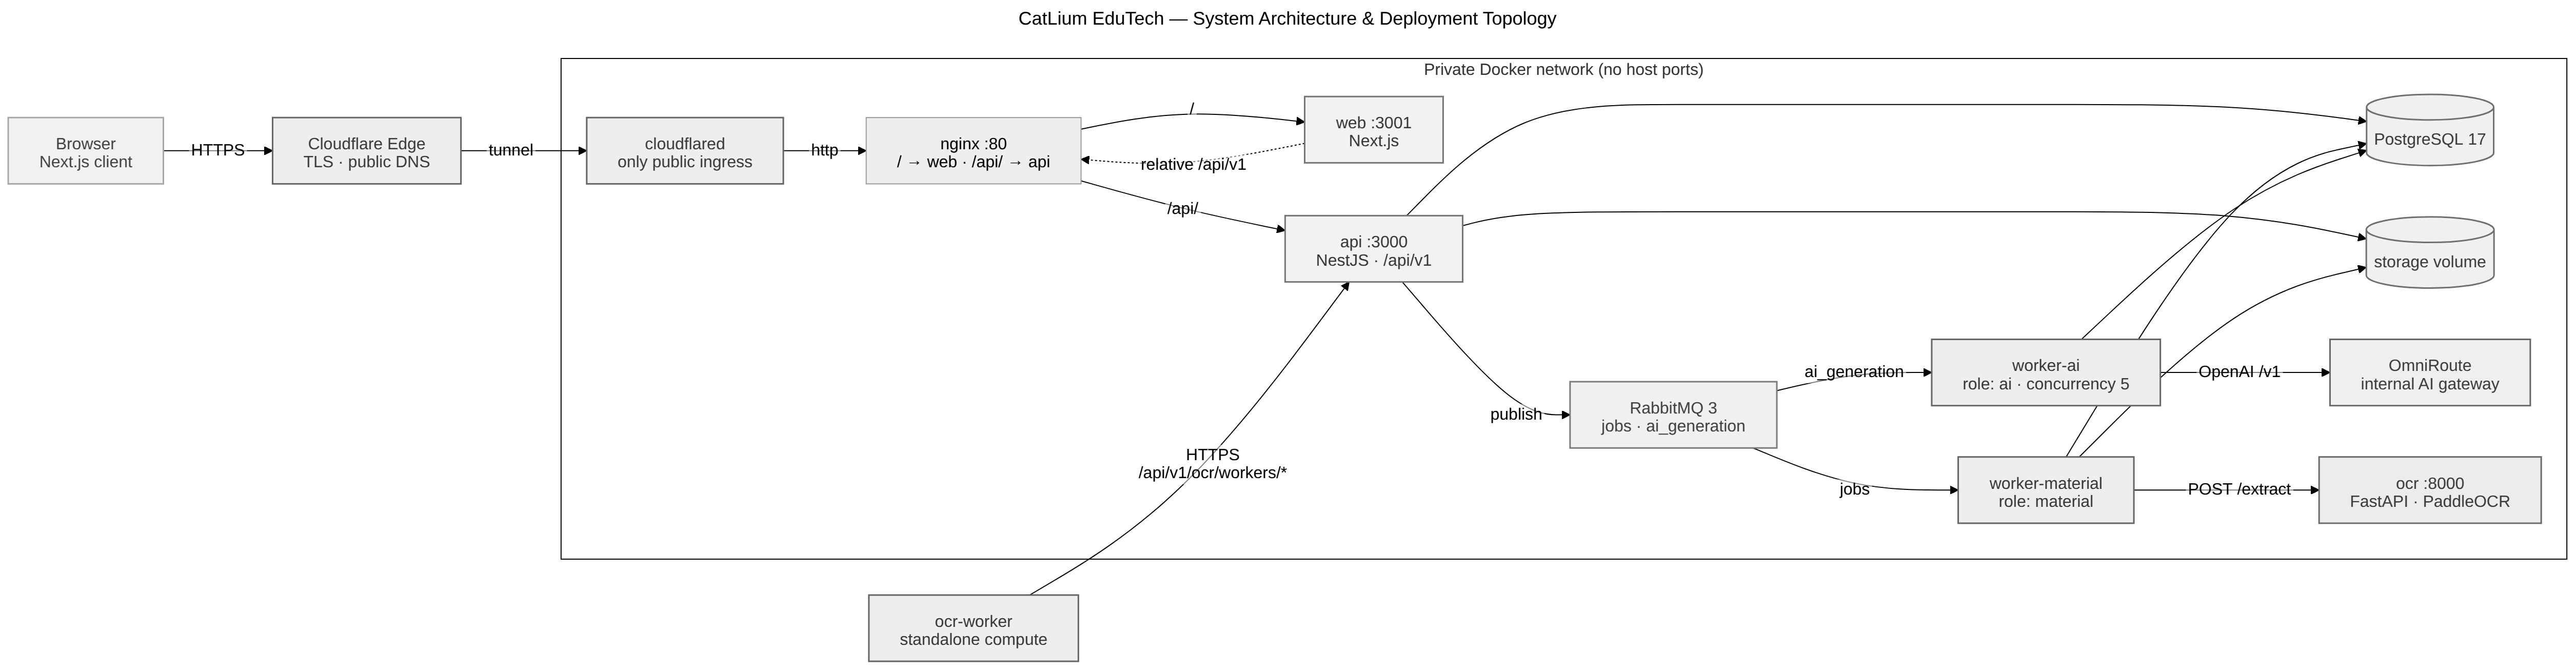
\includegraphics[width=\textwidth]{figures/system-architecture-bw.png}
\caption{System architecture and deployment topology.}
\label{fig:architecture}
\end{figure}

The web application sends its requests to the same origin path
\texttt{/api/v1/\ldots}, which nginx forwards to the API, so browsers never
address internal hosts directly. This single-boundary design means the browser
perceives one same-origin API, and no internal service needs to be publicly
reachable for any user-visible behaviour.

\section{Request Flow and Global Guards}

\noindent Every API request passes a global guard stack registered at the
application root before any controller logic runs:

\begin{enumerate}
  \item \texttt{ThrottlerGuard} --- global rate limit (default 100 requests
  per 60 seconds), tightened to 5 per 60 seconds on authentication routes.
  \item \texttt{CsrfGuard} --- double-submit CSRF check on every cookie-
  authenticated state-changing request.
  \item A global exception filter that normalizes errors into a consistent
  envelope.
\end{enumerate}

\noindent Per-controller, the authorization chain runs
\texttt{AccessTokenGuard $\rightarrow$ TenantGuard $\rightarrow$
RolesGuard $\rightarrow$ PermissionGuard $\rightarrow$ AcademicScope/evaluation
service}, detailed in Chapter~\ref{ch:security} and summarized in
Figure~\ref{fig:permission-model}.

\section{Asynchronous Processing}

\noindent Long-running work is never executed on the request thread. When the
API must perform heavy work it:

\begin{enumerate}
  \item writes a \texttt{jobs} row with status \texttt{queued},
  \item publishes a message to RabbitMQ (or, for coordinator-owned work,
  lets the coordinator sweep adopt it),
  \item returns \texttt{202 Accepted} with the job identifier, and
  \item lets the client poll the job status.
\end{enumerate}

\noindent Two RabbitMQ queues exist: \texttt{jobs} (material processing) and
\texttt{ai\_generation} (all AI operations), with the AI consumer running with
bounded concurrency. AI-related and extraction job types are reserved to
guarded paths; the public job endpoint accepts only material processing and
enhancement types, so a caller cannot forge a request that produces AI output
under another identity. The OCR pipeline is \emph{coordinator-owned}: the
in-API coordinator materialises page-range chunks, hands them to registered
OCR workers under a lease, and aggregates results (Chapter~\ref{ch:features}).
Figure~\ref{fig:ocr-processing} and Figure~\ref{fig:ocr-state} illustrate the
OCR flow and all job/chunk state transitions.

\section{AI Gateway}

\noindent All model calls pass through the internal \texttt{OmniRoute}
gateway, an OpenAI-compatible endpoint. Workers authenticate to the gateway
with their own endpoint key, and no application or worker code calls a cloud
AI provider directly. This keeps the provider switchable and the network
boundary simple.

\section{Health Endpoints}

\noindent The API exposes a health endpoint at
\texttt{GET /api/v1/health} (the global API prefix \texttt{/api/v1} applies to
all controllers). The OCR service exposes its own \texttt{GET /health} route
without an API prefix. These are used by the deployment to report service
liveness.
\chapter{Database Design}
\label{ch:database-design}

\section{Overview}

\noindent PostgreSQL~17 is the single primary database, accessed exclusively
through the Drizzle ORM. The schema is defined in TypeScript in
\texttt{packages/database/src/schema} and deployed as 48 generated SQL
migration files. The current schema contains 47 relations, grouped into the
four families rendered below: (1) identity, tenancy, authentication, and
authorization; (2) academic structure, materials, content, and material
intelligence; and (3) questions, examination, practice, and operational
sub-systems (jobs, OCR registry).

\section{Family 1: Identity, Tenancy, Authentication, and Authorization}

\noindent Figure~\ref{fig:erd-identity} shows the tenancy and authorization
core. Key design properties:

\begin{itemize}
  \item \textbf{Tenant anchor.} \texttt{users} join \texttt{institutes}
  through \texttt{memberships}; a membership is unique per
  (user, institute) and carries an active/deactivated status. All feature
  tables reference \texttt{institute\_id}.
  \item \textbf{Session-bound authentication.} \texttt{auth\_sessions} store a
  SHA-256 hash of the refresh token, an expiry, a revocation timestamp, and a
  \texttt{rotated\_from\_sid} self-link that records rotation lineage.
  \texttt{password\_resets} stores only the bcrypt hash of the one-time secret,
  with a single-use guarantee.
  \item \textbf{Permission catalogue enforced by the schema.}
  \texttt{permissions} rows mirror the typed catalogue in code; \texttt{roles}
  are distinguished as system/institute and institute/platform through CHECK
  constraints and partial unique indexes; \texttt{role\_permissions} and the
  junction \texttt{membership\_roles} implement role-to-permission binding.
  \texttt{\seqsplit{platform\_user\_roles}} binds a user to platform-domain roles,
  fully disjoint from institute membership.
  \item \textbf{Plans.} \texttt{plans} and \texttt{institute\_subscriptions}
  form a minimal lifecycle foundation (starter/growth/institute tiers) without
  billing or feature columns.
\end{itemize}

\begin{figure}[h]
\centering
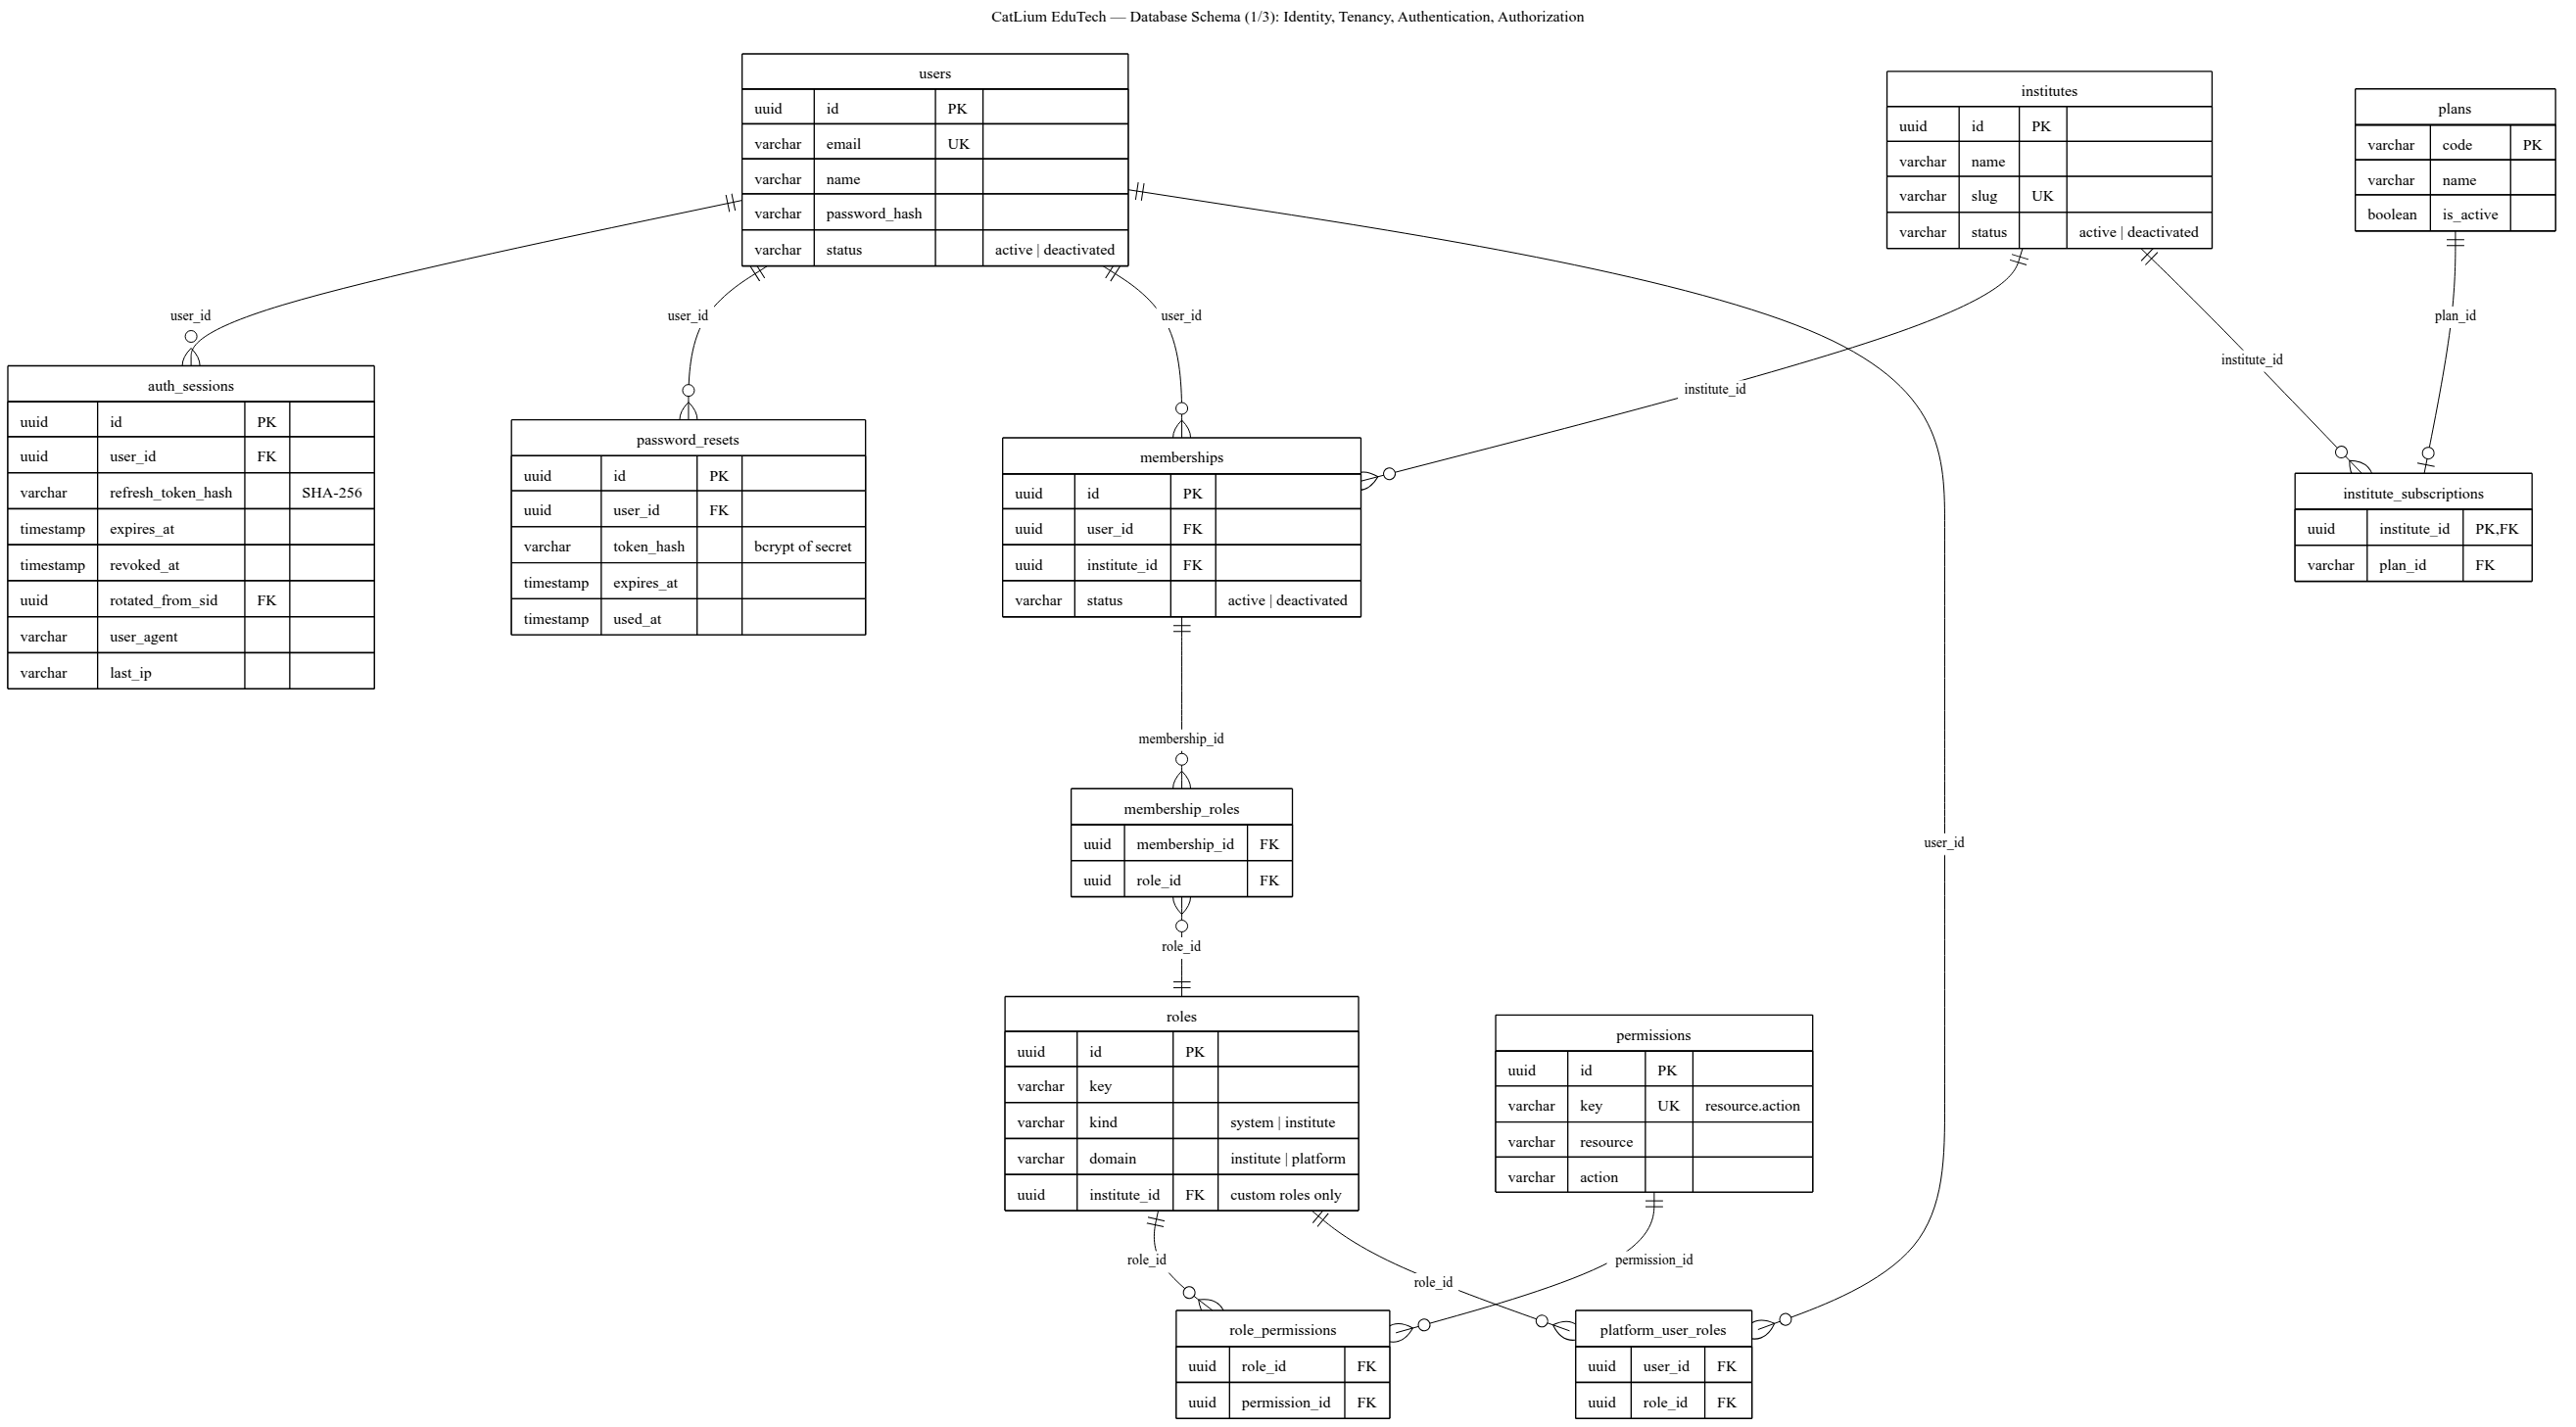
\includegraphics[width=\textwidth]{figures/database-erd-identity-bw.png}
\caption{Database schema --- identity, tenancy, authentication, authorization.}
\label{fig:erd-identity}
\end{figure}

\section{Family 2: Academic Structure, Materials, Content, and Intelligence}

\noindent Figure~\ref{fig:erd-academic-content} shows the academic and
content families. Properties:

\begin{itemize}
  \item \textbf{Scope chain.} \texttt{subjects $\rightarrow$ chapters
  $\rightarrow$ topics} is the single authority for academic scoping; the
  schema enforces consistency with a CHECK on the subject id across the chain.
  \item \textbf{Offerings and assignments.} \texttt{classes} pair with
  \texttt{subjects} in \texttt{class\_subjects} (the offering). Teachers are
  bound to offerings through \texttt{teacher\_assignments}; students are
  placed into a year--class--division through \texttt{student\_placements} and
  may override the inherited subject set with
  \texttt{\seqsplit{student\_subject\_enrollments}} (\texttt{ENROLLED} /
  \texttt{EXCLUDED}).
  \item \textbf{Material vs content.} \texttt{materials} are uploaded
  artifacts with a processing lifecycle and a storage key;
  \texttt{content\_items}/\texttt{content\_versions} are derived, versioned
  study resources whose payload is stored as JSONB with rendered HTML and AI
  context. \texttt{material\_enhancements} (with segment and segment-mapping
  children) store the deterministic structural enrichment of a material.
  \item \textbf{Soft delete.} \texttt{subjects} keeps a nullable
  \texttt{deleted\_at} so academic structure can be archived without
  destroying references.
\end{itemize}

\begin{figure}[h]
\centering
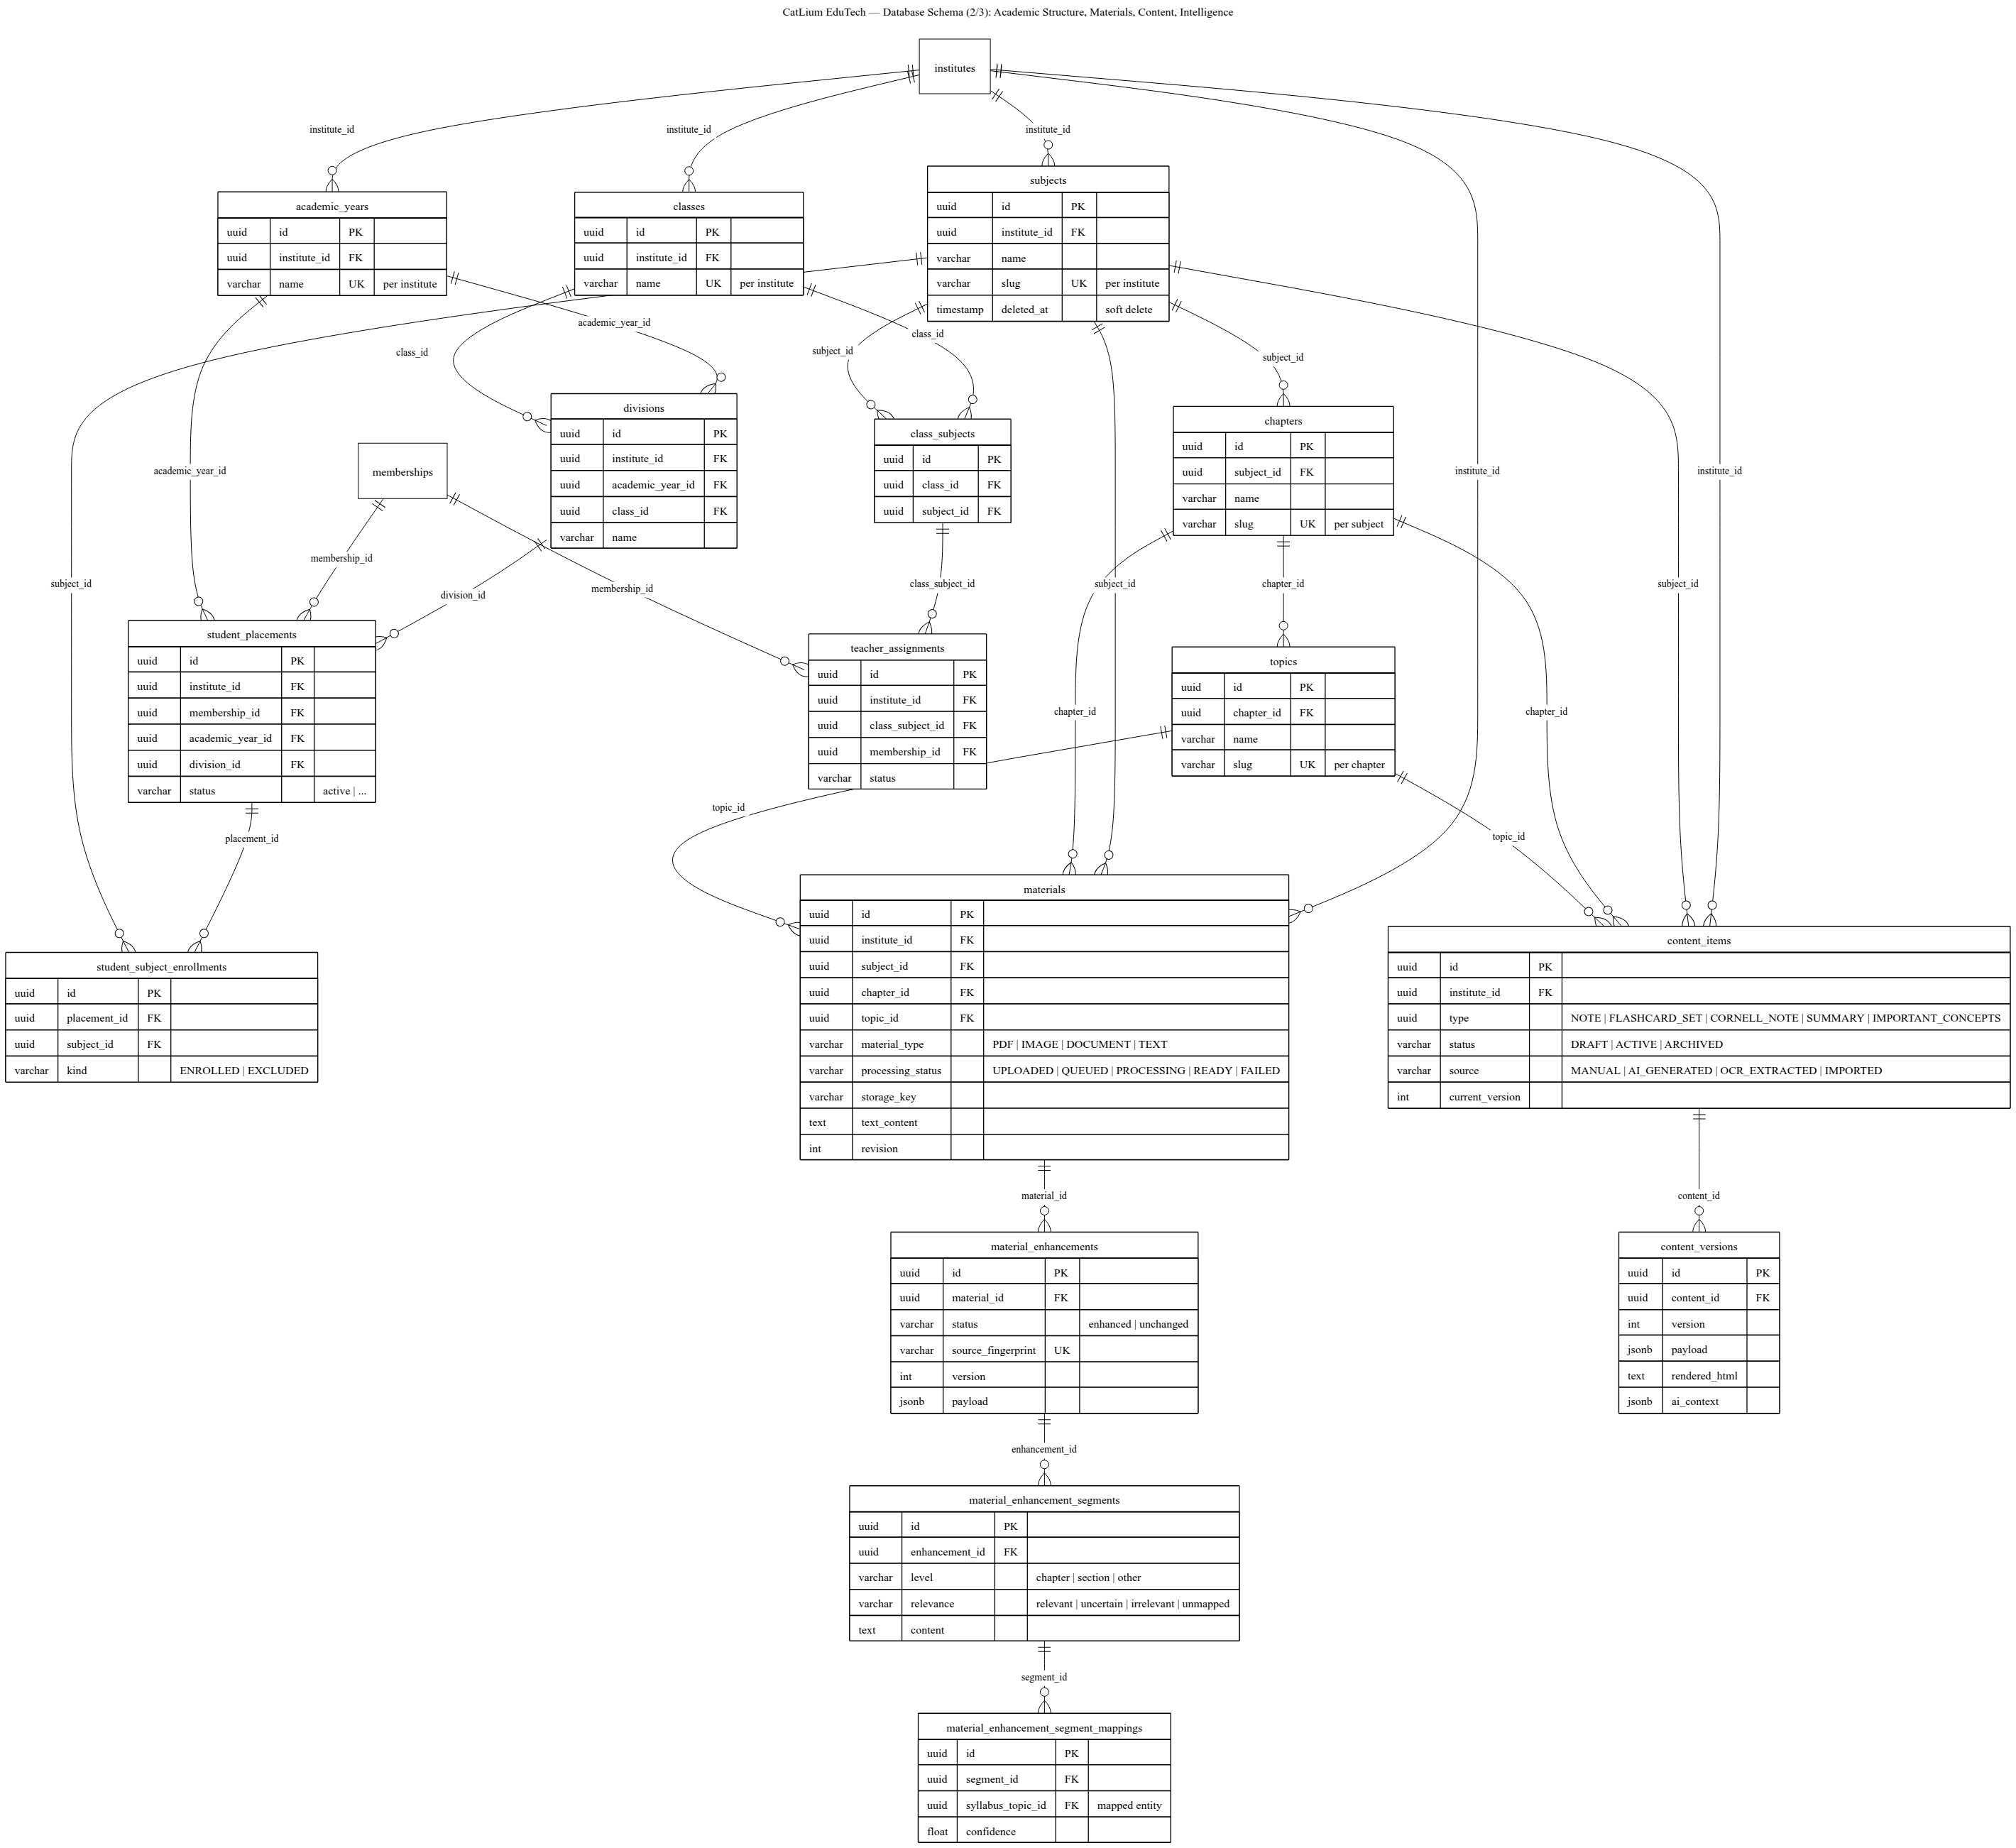
\includegraphics[width=\textwidth]{figures/database-erd-academic-content-bw.png}
\caption{Database schema --- academic structure, materials, content, and
material intelligence.}
\label{fig:erd-academic-content}
\end{figure}

\section{Family 3: Questions, Examination, Practice, and Operations}

\noindent Figure~\ref{fig:erd-operations} shows the question, examination,
practice, and operational families. Properties:

\begin{itemize}
  \item \textbf{Question types as data.} \texttt{question\_types} holds 11
  seeded global starter types plus institute-custom types; \texttt{code} is
  the stable key and \texttt{answer\_format} is copied onto every
  \texttt{questions} row at write time.
  \item \textbf{Immutable attempt snapshot.} \texttt{attempts} records a
  terminal-with-evaluation invariant; \texttt{attempt\_questions} snapshots
  the question stem, type, format, marks, and full server-side payload at
  attempt start; \texttt{attempt\_responses} is the upsertable answer with
  \texttt{is\_correct} and \texttt{marks\_awarded}.
  \item \textbf{Paper artifacts.} \texttt{paper\_patterns} (with
  \texttt{paper\_pattern\_subjects}) drive selection into
  \texttt{question\_papers} and \texttt{assessments} through dedicated
  junction tables that freeze marks, sections, and sort order.
  \item \textbf{Practice.} \texttt{practice\_sessions} support two modes via
  a mode column, and their items/responses are snapshot-like; answers are
  stored with a rating or a correctness flag, never a score.
  \item \textbf{Operational registry.} \texttt{jobs} carries status,
  payload, requester, and completion time with a partial unique index that
  prevents duplicate active AI-generation jobs per source.
  \texttt{workers}/\texttt{ocr\_chunks} implement the distributed OCR
  coordination, with chunk status, \texttt{claimed\_by}, lease expiry, and an
  attempt counter.
\end{itemize}

\begin{figure}[h]
\centering
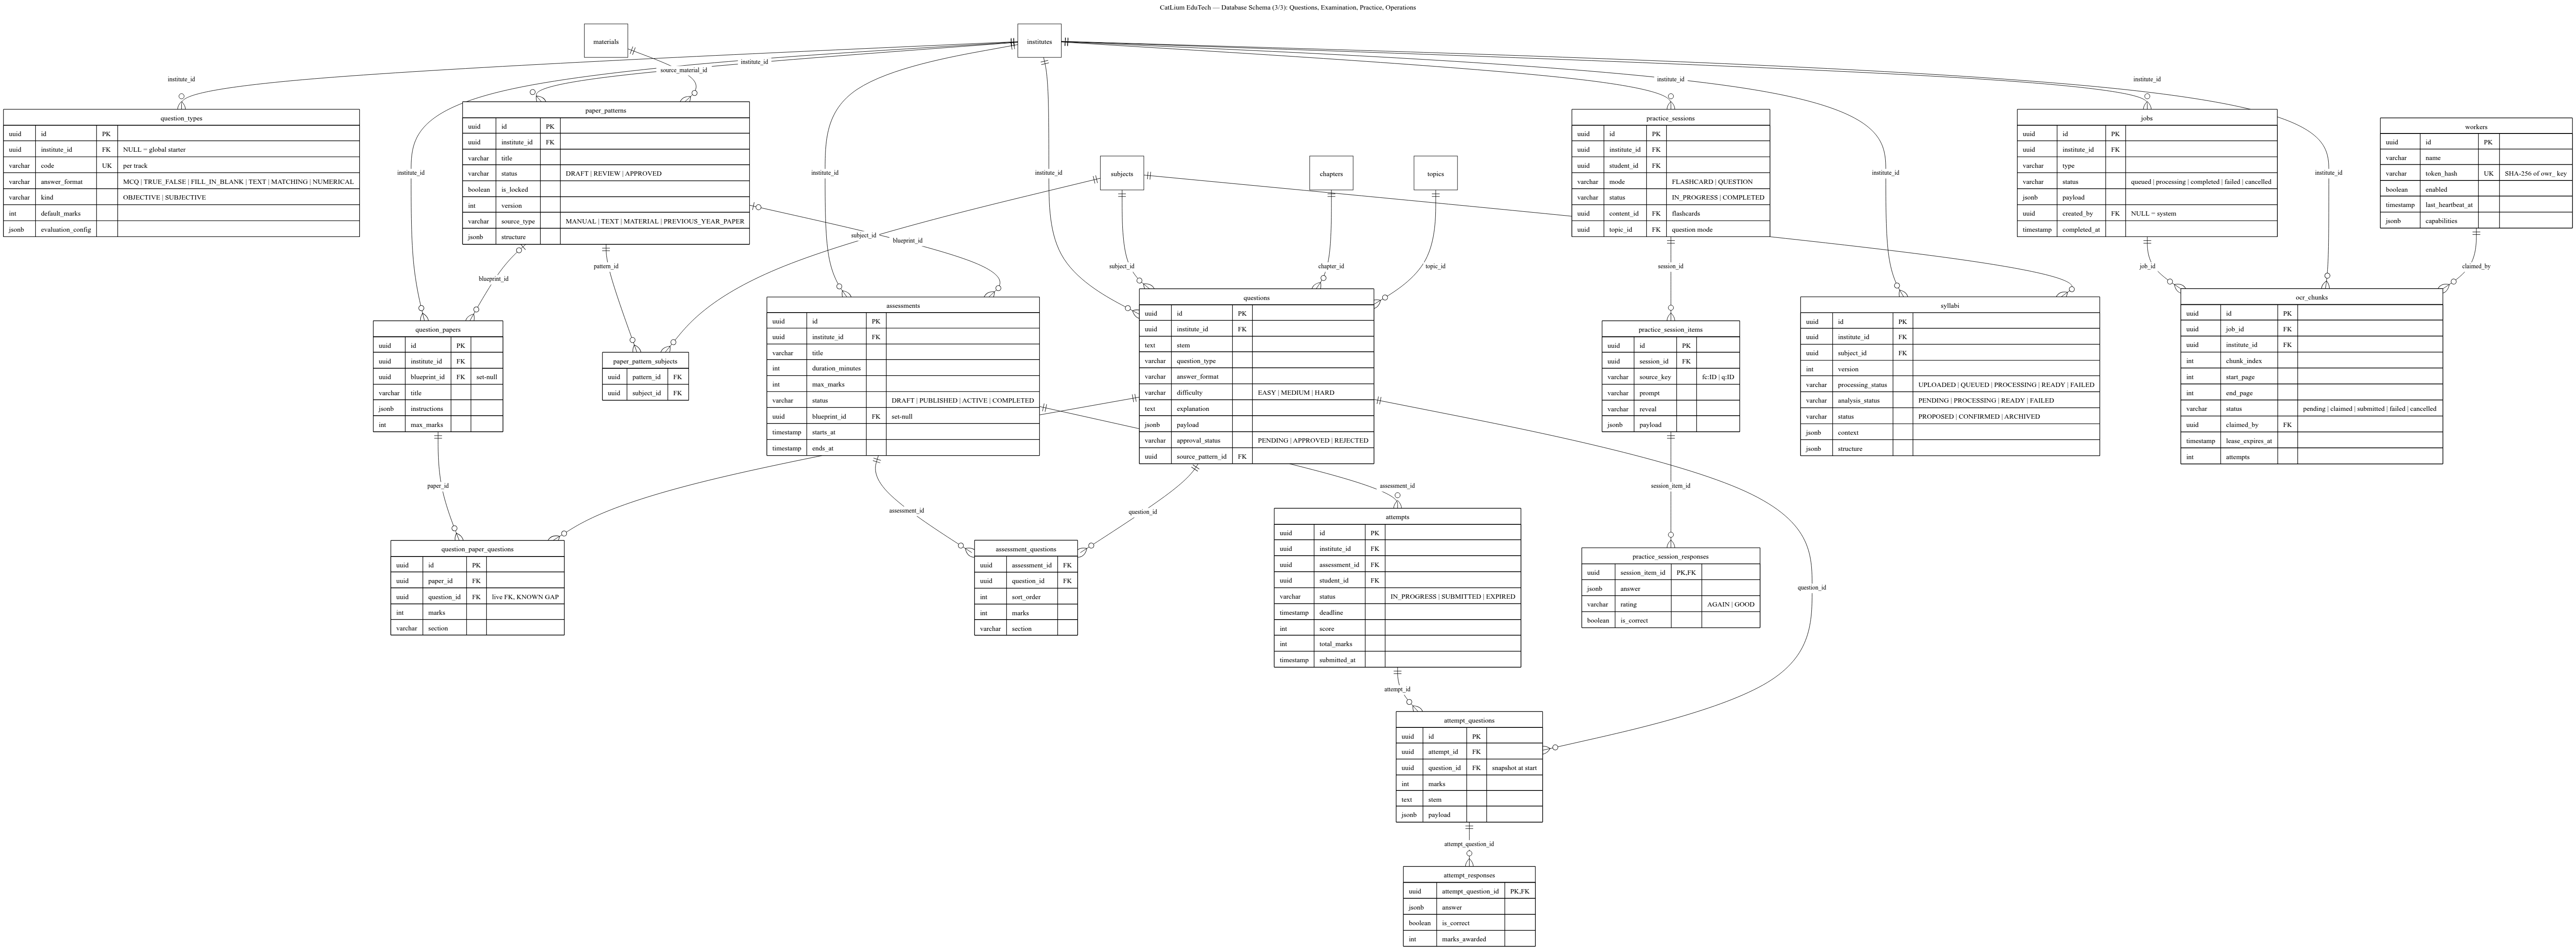
\includegraphics[width=\textwidth]{figures/database-erd-operations-bw.png}
\caption{Database schema --- questions, examination, practice, and operations.}
\label{fig:erd-operations}
\end{figure}

\section{Design Principles Applied}

\noindent Four principles recur across all 47 relations:

\begin{enumerate}
  \item \textbf{Tenant scoping at the row.} Every table that can hold user or
  institute data carries \texttt{institute\_id} so that a forced WHERE clause
  is always available.
  \item \textbf{JSONB for flexible payloads.} Structured-but-variable content
  (question payloads, paper structures, syllabus structures, AI context,
  job payloads) is stored as JSONB and validated at the boundary by Zod
  (TypeScript) or Pydantic (Python), keeping the relational core stable.
  \item \textbf{Snapshot over reference where evaluation depends on it.}
  Attempt question items, practice items, and question-paper junctions copy
  the fields they depend on, so later edits to a source question cannot
  silently change an in-flight or historical artifact.
  \item \textbf{Database-enforced invariants.} Partial unique indexes (one
  in-progress attempt per assessment+student, one open practice session per
  source, no duplicate active generation per source) turn races into
  deterministic \texttt{409} conflicts; \texttt{FOR UPDATE SKIP LOCKED} makes
  the OCR chunk claim safe under concurrency.
\end{enumerate}
\chapter{Security and Authorization Architecture}
\label{ch:security}

\section{Security Goals}

\noindent The security goals of the platform are: (i) tenant isolation that
holds at the enforcement layers by default; (ii) session security that resists
token theft and replay; (iii) authorization that evaluates current database
state instead of cached claims; and (iv) a contained attack surface in which
nothing user-facing depends on a publicly reachable internal service.

\section{Authentication}

\sectionmark{Authentication}
\noindent Authentication is cookie-based, following the OWASP guidance for
session management~\cite{owaspsession}. The flow is shown in
Figure~\ref{fig:auth-sequence}.

\begin{figure}[h]
\centering
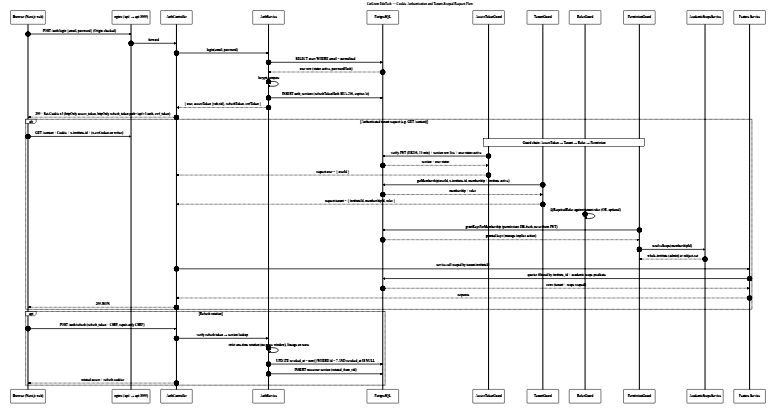
\includegraphics[width=\textwidth]{figures/authentication-sequence-bw.png}
\caption{Cookie authentication and the tenant-scoped request flow.}
\label{fig:auth-sequence}
\end{figure}

\subsection{Cookies and tokens}

\noindent Three cookies are issued:

\begin{itemize}
  \item \texttt{access\_token} --- httpOnly, path \texttt{/}, short-lived
  (default 15 minutes). It is a JWT, signed HS256, whose payload carries only
  \texttt{\{sub, sid\}}: the subject (user id) and the session id. Permissions
  are never placed in the token.
  \item \texttt{refresh\_token} --- httpOnly, path \texttt{/api/v1/auth},
  long-lived (default 30 days, sliding). Only its SHA-256 hash is stored in
  \texttt{auth\_sessions}.
  \item \texttt{csrf\_token} --- not httpOnly, path \texttt{/}, for the
  double-submit CSRF scheme.
\end{itemize}

\noindent SameSite defaults to \texttt{lax}; the \texttt{Secure} attribute is
enabled in production. In production the \texttt{JWT\_SECRET} must be present
at boot or the service refuses to start.

\subsection{Access token validation}

\noindent The \texttt{AccessTokenGuard} verifies the JWT, requires a
\texttt{sid}, loads the referenced \texttt{auth\_sessions} row, and checks that
the session is live (not revoked, not expired, owned by \texttt{sub}) and that
the user's status is still \texttt{active}. Revocation or deactivation
therefore takes effect on the very next request; there is no residual window.

\subsection{Strict refresh rotation}

\noindent Refresh rotation is strictly one-time. On \texttt{POST}
\texttt{/auth/refresh} the service atomically claims the session with
\texttt{UPDATE auth\_sessions SET revoked\_at = now() WHERE id = ? AND
revoked\_at IS NULL AND refresh\_token\_hash = ?}; only the single winning
request mints the successor row. There is no grace window --- re-rotation of a
spent token is treated as replay. If a spent token is presented, the service
walks the \texttt{rotated\_from\_sid} lineage and revokes the whole family; a
wrong token against a live row is treated as suspected theft and revokes that
session. \texttt{POST /auth/refresh} is also CSRF-guarded and CSRF-repair-only.
Logout is refresh-session aware: it revokes by the refresh session id first,
falls back to the access \texttt{sid} claim, and clears the cookies
unconditionally. Users may list their sessions and revoke any single one or
all but the current session.

\subsection{CSRF protection}

\noindent The double-submit scheme is registered as a global guard. On every
state-changing (non-GET), cookie-authenticated request, the client must echo
the \texttt{csrf\_token} cookie in the \texttt{x-csrf-token} header; a
missing or mismatched value yields \texttt{403}. Requests without an access
cookie are exempt (there is no session to protect --- this is also the seam
that lets cookie-free worker protocols operate), and GET/HEAD/OPTIONS are
always allowed. The custom \texttt{x-institute-id} header doubles as
defense-in-depth, since cross-origin calls must pass browser CORS
preflight to send it.

\subsection{Login protection}

\noindent \texttt{POST /auth/login} is throttled (5 per 60 seconds), rejects
sessions for deactivated accounts, returns uniform responses that do not
enumerate users, and validates that the request Origin matches the Host.
Passwords are hashed with bcrypt (cost~12 for new accounts).

\subsection{Password reset}

\noindent The reset flow issues a one-time token (identifier plus a 32-byte
secret), stores only the bcrypt hash of the secret, expires it after 30
minutes, and atomically consumes it via a \texttt{used\_at} guard. A
successful reset revokes every session of the user. Delivery of the reset
token is an integration seam (provider not yet wired), and the raw token is
never logged.

\section{Authorization}

\noindent Authorization is evaluated per request and in layers. The complete
decision chain is rendered in Figure~\ref{fig:permission-model};
the academic-scope engine is detailed in Figure~\ref{fig:academic-scope}.

\begin{figure}[h]
\centering
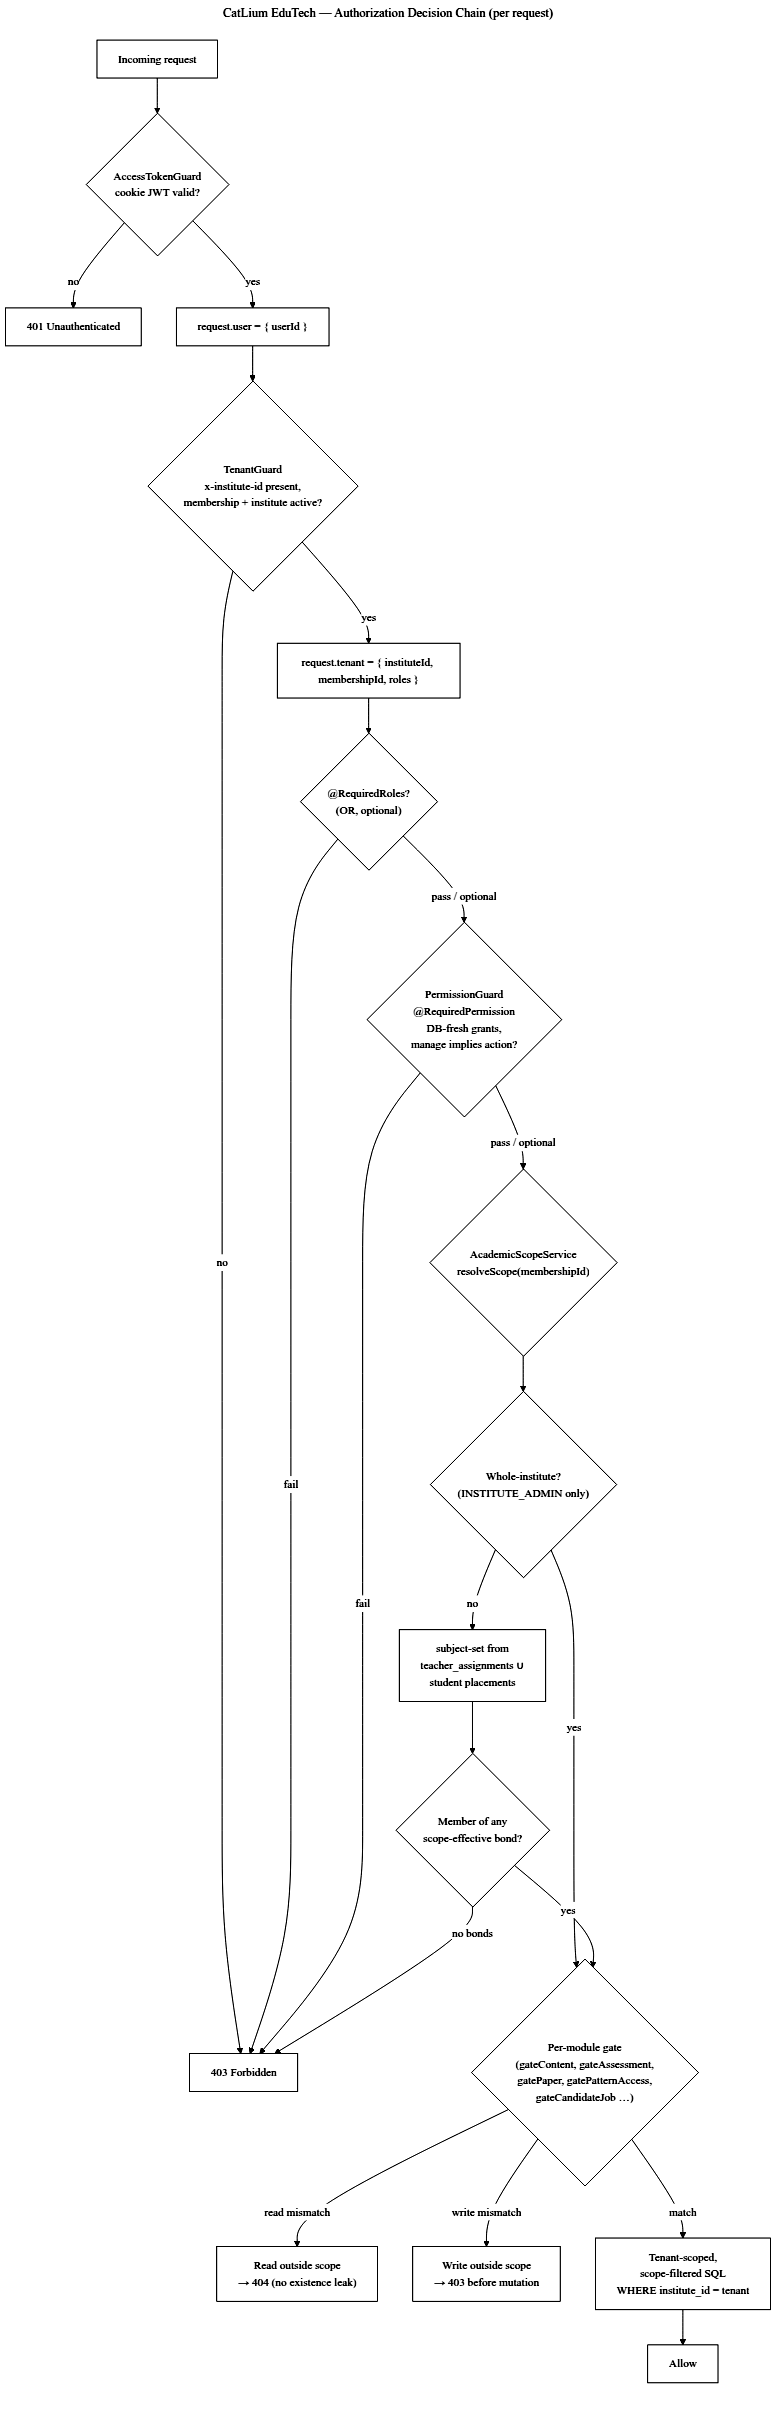
\includegraphics[width=\textwidth]{figures/permission-model-bw.png}
\caption{Authorization decision chain for a tenant-scoped request.}
\label{fig:permission-model}
\end{figure}

\begin{figure}[h]
\centering
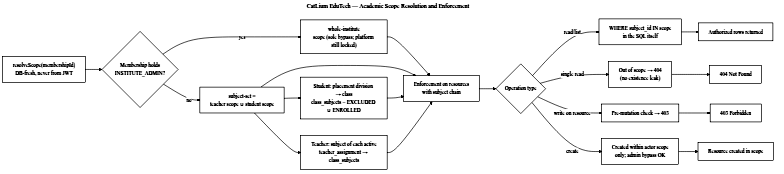
\includegraphics[width=\textwidth]{figures/academic-scope-bw.png}
\caption{Academic scope resolution and enforcement (reads 404, writes 403).}
\label{fig:academic-scope}
\end{figure}

\subsection{The guard chain}

\noindent For tenant-scoped endpoints the chain is
\texttt{AccessTokenGuard} $\rightarrow$ \texttt{TenantGuard} $\rightarrow$
\texttt{RolesGuard} $\rightarrow$ \texttt{PermissionGuard}. Public endpoints
and the platform plane use
lighter chains (see below). A permission check is
\emph{DB-fresh}: the \texttt{PermissionGuard} loads the membership's granted
keys by joining memberships $\rightarrow$ roles $\rightarrow$ role permissions
$\rightarrow$ permissions and evaluates against the declared
\texttt{@RequiredPermission} keys; \texttt{R.manage} implies any action of
resource \texttt{R}. Nothing about authorization is cached across requests,
so removing a role or permission takes effect on the next request.

\subsection{The permission catalogue}

\noindent The catalogue is a single typed map in code (mirrored into the
\texttt{permissions} table at every API boot) with 83 keys over 19 resources.
Institute-domain resources \texttt{subjects}, \texttt{chapters},
\texttt{topics}, \texttt{content}, \texttt{materials}, \texttt{syllabus},
\texttt{questions}, \texttt{question-types}, \texttt{paper-patterns},
\texttt{question-papers}, \texttt{assessments}, \texttt{attempts},
\texttt{practice}, \texttt{exports}, \texttt{jobs}, \texttt{users}, and
\texttt{roles} each carry the actions \texttt{read}, \texttt{create},
\texttt{update}, \texttt{delete} (where an endpoint exists), and
\texttt{manage}; the platform domain carries \texttt{institutes} and
\texttt{ocr-workers}. Keys are explicit and without wildcards; unknown keys
resolve to \texttt{false}. The full catalogue is reproduced in
Appendix~\ref{app:permissions}.

\subsection{Built-in roles}

\begin{itemize}
  \item \texttt{INSTITUTE\_ADMIN} holds \texttt{manage} on every institute
  resource (17 keys) and resolves to whole-institute academic scope;
  \item \texttt{TEACHER} holds 47 institute keys covering content,
  materials, structure, questions, patterns, papers, assessments, reads on
  attempts, and job management;
  \item \texttt{STUDENT} holds 14 read-oriented keys over structure, content,
  syllabi, and assessments plus attempt/practice self-actions;
  \item \texttt{SUPER\_ADMIN} holds all nine platform keys and is never a
  membership role; the platform plane is enforced by \texttt{PlatformGuard},
  which is independent of \texttt{x-institute-id}.
\end{itemize}

\noindent Institute admins create custom roles from the institute catalogue
(max 128 keys per role). Custom roles never receive platform permissions, and
an actor cannot modify a role they currently hold (self-escalation guard).

\subsection{Academic scope}

\noindent A permission alone never grants access: the resource's subject (or
its absence) must also match the actor's scope. The
\texttt{AcademicScopeService} resolves the actor's subject set from \emph{current
database state}: for teachers, the union of subjects over their active
\texttt{teacher\_assignments}; for students, the class-subject set of their
placement's division, minus \texttt{EXCLUDED} and plus \texttt{ENROLLED}
enrollments. An actor with no bonds gets an empty set (default deny).
\texttt{INSTITUTE\_ADMIN} is the sole whole-institute bypass and never escapes
the institute.

\subsection{Enforcement points and status codes}

\noindent Reads are scoped in the SQL itself: list queries filter by the
subject predicate, and a single-resource read out of scope returns
\texttt{404} (no existence leak). Writes perform an explicit resource check
\emph{before} mutation and return \texttt{403}. Ownership layers supplement
scope on DRAFT and PENDING resources (owner-and-admin-only until shared).
Module gate helpers (\texttt{gateContent}, \texttt{gateAssessment},
\texttt{gatePaper}, \texttt{gatePatternAccess}, \texttt{gateCandidateJob})
apply the same 404-read/403-write contract across their modules.

\section{Internal Service Authentication}

\noindent Internal HTTP calls use a shared \texttt{x-internal-api-key} header
(sent by the API to the OCR service when so configured). Distributed OCR
workers authenticate per worker: \texttt{x-worker-id} plus a bearer
\texttt{owr\_...} key whose SHA-256 hash is stored on the worker row and
compared in constant time. Workers call the AI gateway with a standard
\texttt{Authorization: Bearer} endpoint key. There is no direct cloud AI SDK
call from application code.

\section{Summary of Security Decisions}

\noindent The security and authorization design was settled in seven recorded
architectural decisions (D1--D7) and a session-hardening list (F1--F6), all
implemented and validated:

\begin{center}
\small
\begin{tabular}{@{}p{0.7cm}p{5.1cm}p{8.2cm}@{}}
\toprule
\textbf{Dec.} & \textbf{Decision} & \textbf{Implementation summary} \\
\midrule
D1 & Permission model & Explicit \texttt{resource.action} keys, default-deny,
\texttt{manage} implication, no wildcards, catalogue---table consistency check. \\
D2 & Role/permission storage & \texttt{roles}, \texttt{permissions},
\texttt{role\_permissions}, and \texttt{membership\_roles} relations with
schema CHECKs and partial unique indexes. \\
D3 & Platform plane & \texttt{SUPER\_ADMIN} via
\texttt{platform\_user\_roles}, disjoint from membership; \texttt{PlatformGuard}
independent of tenant header. \\
D4 & Academic structure & Years, classes, divisions, class--subject offerings;
offerings at class level. \\
D5 & Assignments & Teacher assignments and student placements at offering
granularity; no division-level subjects. \\
D6 & Resource scope & Subject chain (with optional offering-level scope in
design) + default-deny; admin bypass is the sole exception; ownership
stages O1--O3. \\
D7 & Session hardening & F1--F6: session-bound access tokens, strict one-time
rotation with lineage revocation, refresh-aware logout, global double-submit
CSRF with origin check, status-gated refresh, defined cookie and retention
posture. \\
\bottomrule
\end{tabular}
\end{center}

\noindent A documentation-led security audit (Phase~M) verified the
implementation against the threat model and remediated the findings: an export
endpoint that could expose answer keys was closed (HIGH), a cross-institute
OCR/enhancement job adoption path was fixed (MEDIUM), job ownership was
recorded (LOW), stale institute context was cleaned on logout (LOW), and
documentation was brought in line with the code.
\chapter{Core Features and Workflows}
\label{ch:features}

\begin{center}
\textit{This chapter explains each implemented feature area --- its purpose,
data model, workflow, and integration with the authorization model of
Chapter~\ref{ch:security}.}
\end{center}

\vspace*{\fill}
\clearpage
\section{Identity and Tenancy}

Users, institutes, memberships, roles, and permissions form the identity core.
There is no public self-registration: institute admins create users and
memberships, so every account arrives with an institute context and role. A
user may belong to several institutes; the client pins the active institute
(\texttt{x-institute-id}) per request and the browser stores it locally,
clearing it on logout or an unauthorized response. The membership picker
returns the user's memberships together with their resolved institute-domain
permission keys, so the web client can adapt its UI to what the user may
actually do. Institute lifecycle (create/deactivate) is modelled as
platform-plane work for a future \texttt{SUPER\_ADMIN} surface; role
management and user provisioning are institute-admin features today.

\section{Academic Structure and Academic Scope}

The academic module models \texttt{academic\_years}, \texttt{classes},
\texttt{divisions}, \texttt{subjects}, \texttt{chapters}, \texttt{topics}, and
the offering table \texttt{class\_subjects}. Teacher assignments bind a
membership to an offering (class--subject) for a term; student placements bind
a membership to a year--class--division and can be refined by explicit subject
enrollments. This structure is the input to
\texttt{\seqsplit{AcademicScopeService}}
(Figure~\ref{fig:academic-scope-resolution}): teachers and students get a
subject set
from their assignments/placements, from which every content query is scoped.
Structural administration (structure creation, assignment changes) is admin
work; content visibility derived from it is enforced per query.

\section{Materials and the OCR Pipeline}

\sectionmark{Materials and OCR}
Materials are uploaded as PDF, image, or document files (chunked upload for
large files, up to 20~MB total), or entered as plain text. Each material row
tracks \texttt{processing\_status} (\texttt{UPLOADED} $\rightarrow$
\texttt{QUEUED} $\rightarrow$ \texttt{PROCESSING} $\rightarrow$ \texttt{READY} |
\texttt{FAILED}) and a revision number.
Processing is asynchronous and coordinator-owned: the in-API coordinator
adopts queued \texttt{MATERIAL\_PROCESS} jobs, splits the source into page
chunks of default size ten, and lets registered OCR workers claim chunks under
a lease. Figure~\ref{fig:ocr-processing} and Figure~\ref{fig:ocr-processing-part2}
show the distributed flow and Figure~\ref{fig:ocr-state} and Figure~\ref{fig:ocr-state-part2}
the job/chunk state machines.

\begin{sidewaysfigure}[p]
\centering
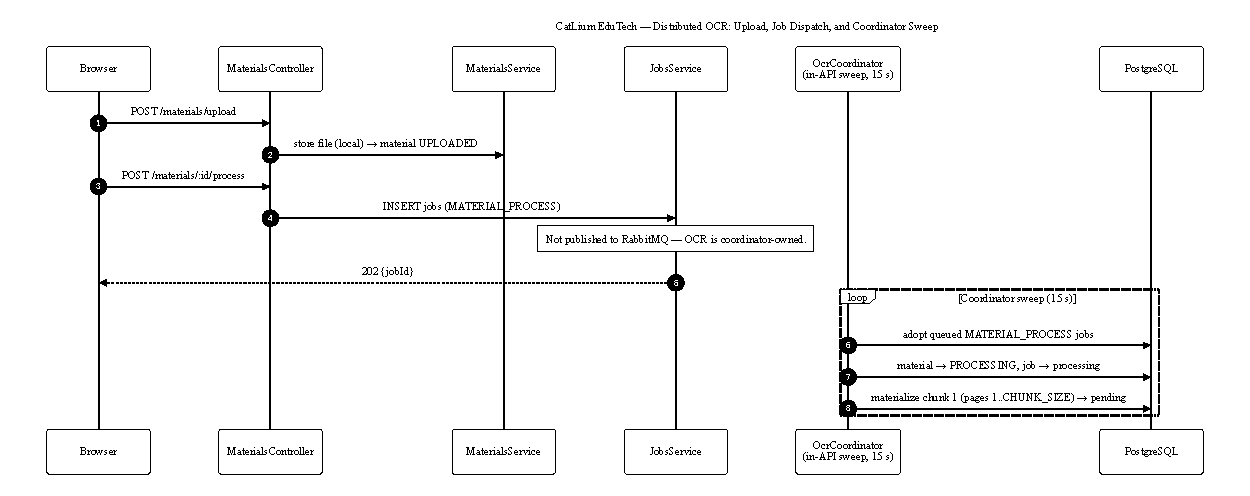
\includegraphics[width=711.5pt]{figures/ocr-flow-coordinator-sequence-bw.pdf}
\caption{Distributed OCR material processing, part 1: upload, job dispatch,
and the coordinator sweep.}
\label{fig:ocr-processing}
\end{sidewaysfigure}

\begin{figure}[p]
\centering
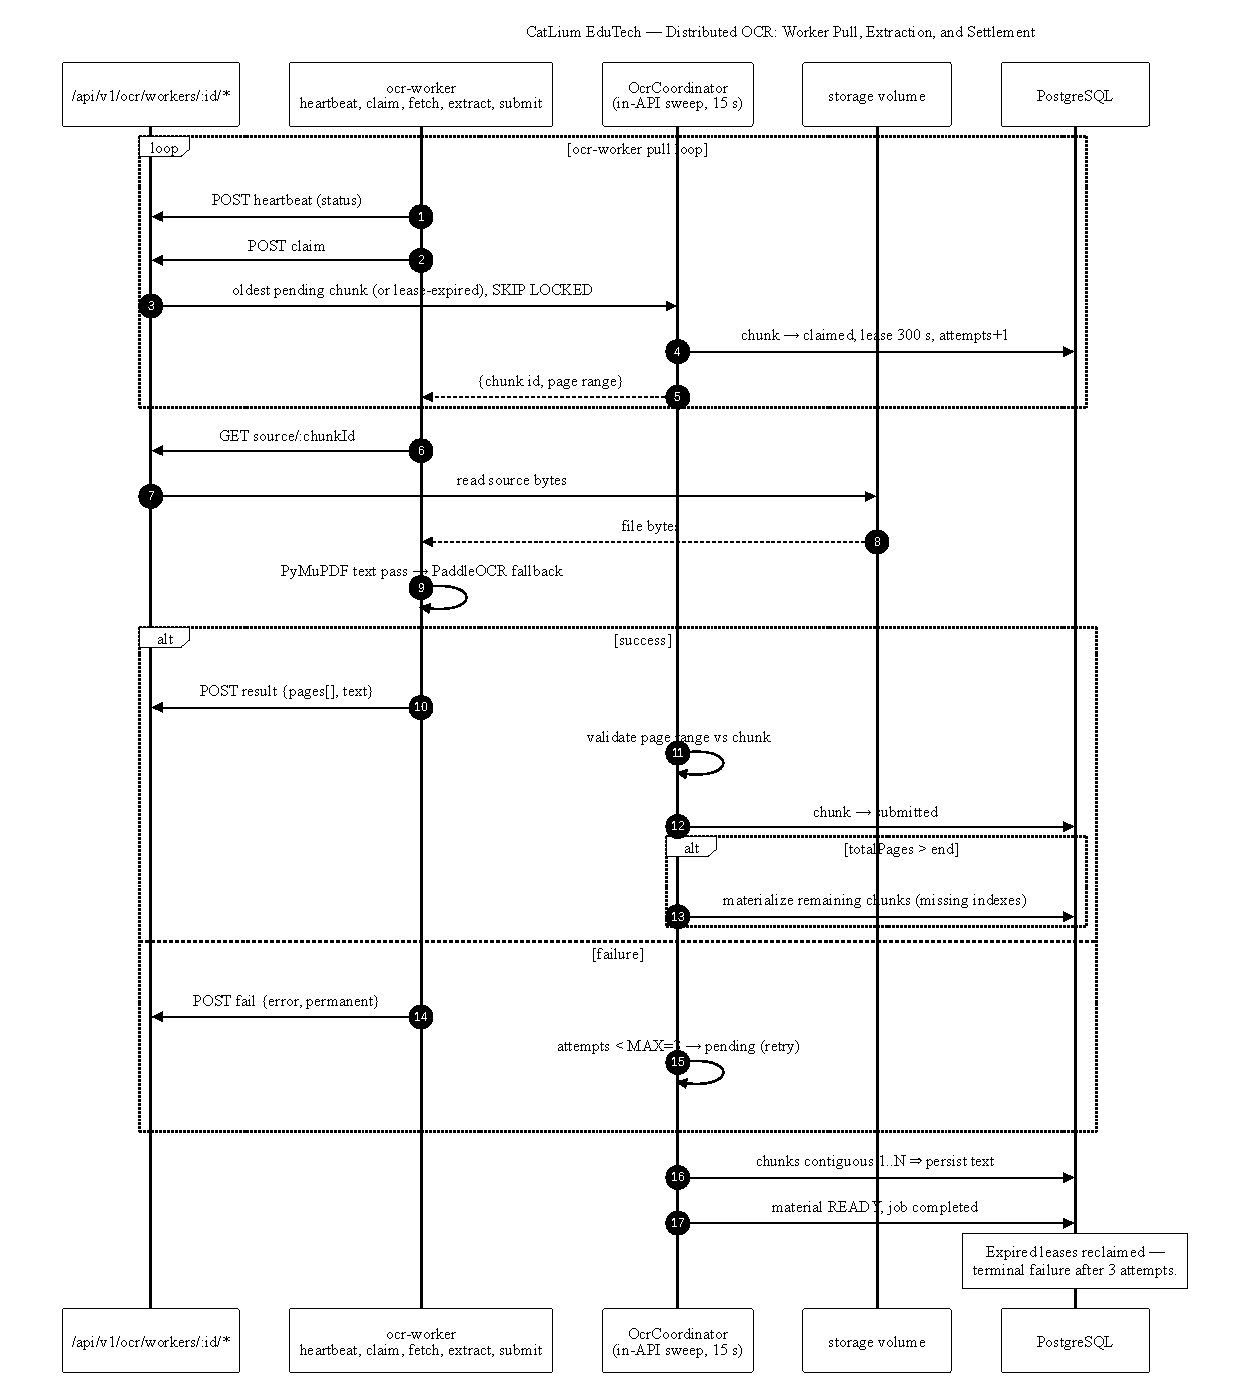
\includegraphics[width=436.5pt]{figures/ocr-flow-worker-sequence-bw.pdf}
\caption{Distributed OCR material processing, part 2: worker pull, extraction,
and settlement.}
\label{fig:ocr-processing-part2}
\end{figure}

\begin{sidewaysfigure}[p]
\centering
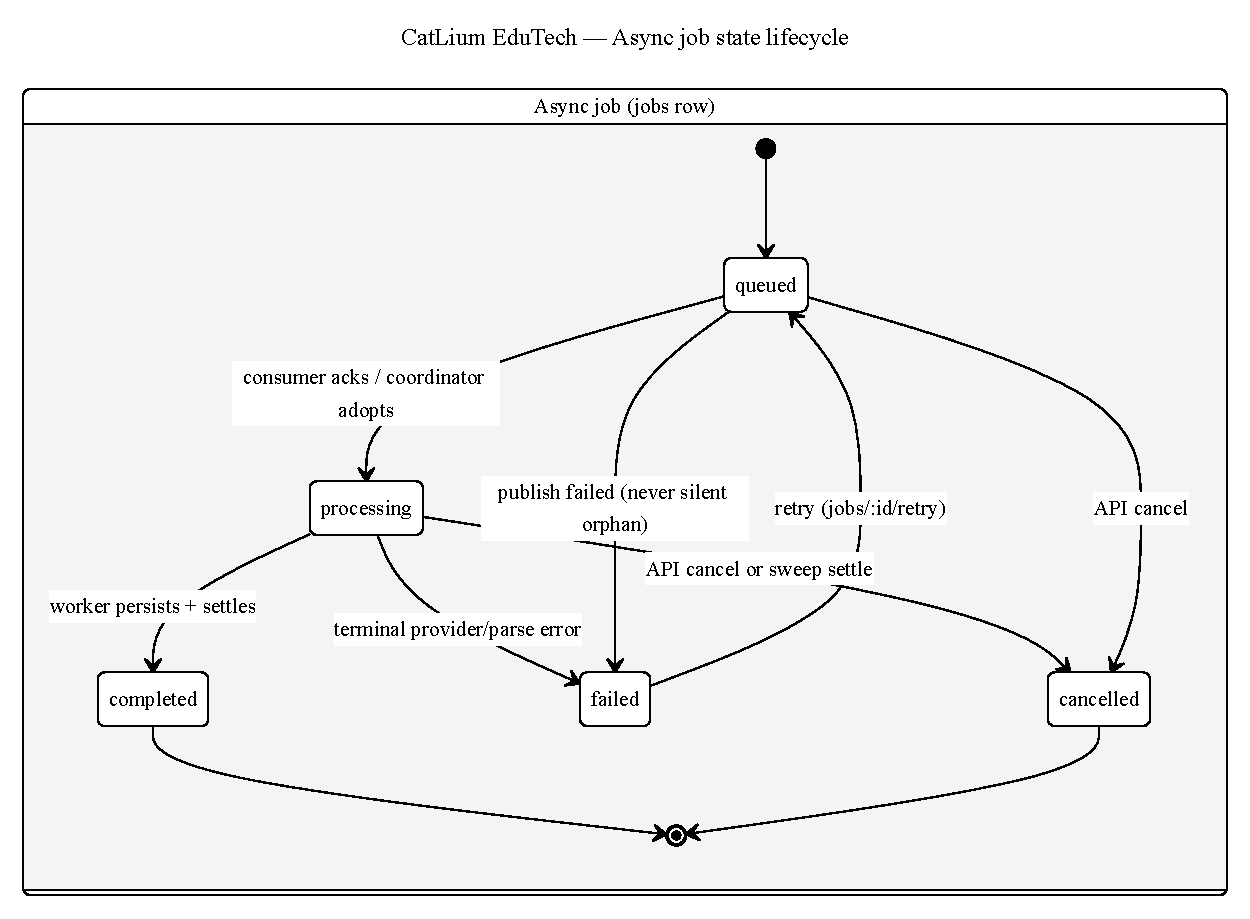
\includegraphics[width=544.9pt]{figures/state-job-lifecycle-bw.pdf}
\caption{Job state lifecycle.}
\label{fig:ocr-state}
\end{sidewaysfigure}

\begin{sidewaysfigure}[p]
\centering
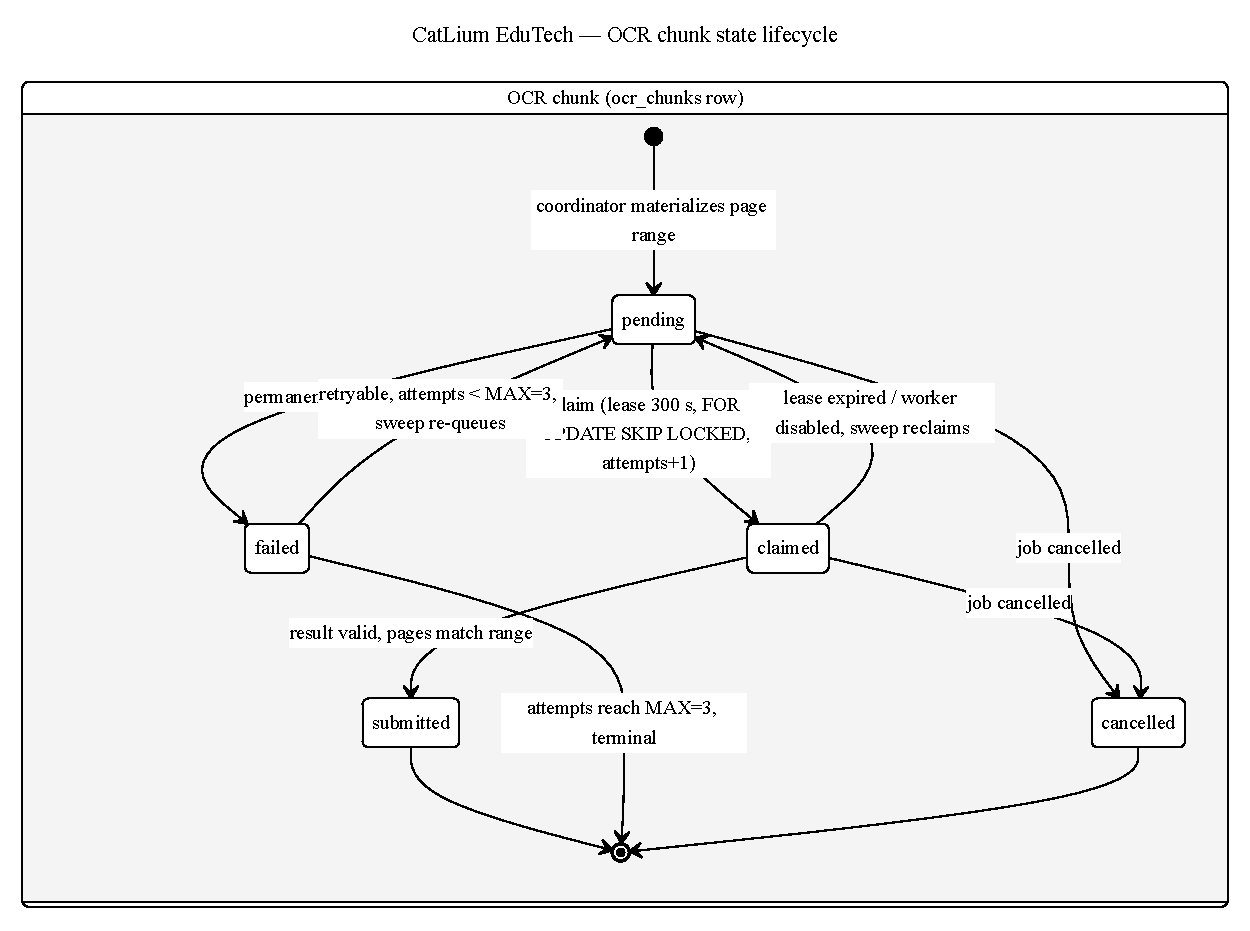
\includegraphics[width=537.6pt]{figures/state-chunk-lifecycle-bw.pdf}
\caption{OCR chunk state lifecycle.}
\label{fig:ocr-state-part2}
\end{sidewaysfigure}

For each page an OCR worker first tries PyMuPDF embedded text; a page with at
least five usable characters is accepted as-is, otherwise the page is
rasterised and fed to PaddleOCR. Extraction is followed by a deterministic
character-normalization pass. Worker claims are granted with
\texttt{FOR UPDATE SKIP LOCKED}; a lease (default 300 seconds) is renewed by
heartbeat, and the coordinator sweep (default every 15 seconds) reclaims
expired or disabled-worker claims, retries failed chunks while the attempt
count is below three, and settles cancellations. When all chunks of a
material are submitted and the pages are contiguous, the aggregate text is
persisted and the material becomes \texttt{READY}, which unlocks downstream
reuse: page-level text is viewable and users can submit per-page corrections
that re-apply over the extracted text. Workers authenticate per worker
(\texttt{owr\_...} keys against a SHA-256 hash); the worker-facing endpoints
are throttled and platform-gated.

\section{Syllabus Intelligence}

A syllabus document is uploaded (text or file) and processed to text, then
analysed by an AI job (\texttt{AI\_ANALYZE\_SYLLABUS}) that produces a
per-subject \texttt{structure} (chapters with their topics) and a
\texttt{context} (program, course, academic year, objectives, learning
outcomes, units and their scope). The lifecycle runs
\texttt{PROPOSED $\rightarrow$ CONFIRMED} (with \texttt{ARCHIVED}), and the
analysis can be re-run; a \texttt{CONFIRMED} syllabus is never silently
overwritten, so teachers can confirm a version and regenerate without data
loss. Each subject's syllabus carries a version number (\texttt{max+1} on
replacement) and both processing and analysis three-state machines.

\section{Material Intelligence (Deterministic Enrichment)}

In addition to AI, materials receive a deterministic structural enrichment
(\texttt{\seqsplit{material\_enhancements}}): a pure algorithmic pass over the extracted
pages that classifies every block (heading, paragraph, list, table, equation,
other) and keeps or marks segments (chapter/section) with a relevance level and
a confidence-scored mapping to syllabus topics. This pass is idempotent --- a
source fingerprint (checksum of extracted text and revision) prevents
duplicate re-enrichment --- and never modifies the raw extraction; excluded
blocks retain their original text and a reason. Enrichment is coordinator-owned
like OCR and triggered by OCR completion, corrections, text sources, or manual
re-enhancement.

\section{Study Content and AI Generation}

Content items are typed (\texttt{NOTE}, \texttt{\seqsplit{FLASHCARD\_SET}},
\texttt{\seqsplit{CORNELL\_NOTE}}, \texttt{SUMMARY},
\texttt{\seqsplit{IMPORTANT\_CONCEPTS}}), carry
a source (\texttt{MANUAL} | \texttt{AI\_GENERATED} |
\texttt{\seqsplit{OCR\_EXTRACTED}}
| \texttt{IMPORTED}), a status (\texttt{DRAFT} | \texttt{ACTIVE} |
\texttt{ARCHIVED}), and versioned payloads in \texttt{content\_versions} that
store the rendered HTML and AI context. Content availability is scoped by the
subject chain and the actor's academic scope.

AI generation (Figure~\ref{fig:ai-generation} and
Figure~\ref{fig:ai-generation-part2}) is an asynchronous pipeline:
the API writes a \texttt{jobs} row and publishes to the \texttt{ai\_generation}
queue; a Python worker with bounded concurrency resolves the eligible READY
source materials, assembles a bounded context budget, calls the model through
the OmniRoute gateway in chunks, validates each response against a strict
Pydantic schema for the requested artifact, aggregates and deterministically
de-duplicates, then persists the produced items AI-generated with provenance
(source type, source id, exact material revisions used). Generation on a topic
with no READY material enqueues a starter-material job whose
dependent-resources release the planned children, so a topic's generation
waits until it has usable sources. Generated content is versioned in place
(with REGENERATION change types) and never duplicated per topic/type.

\begin{sidewaysfigure}[p]
\centering
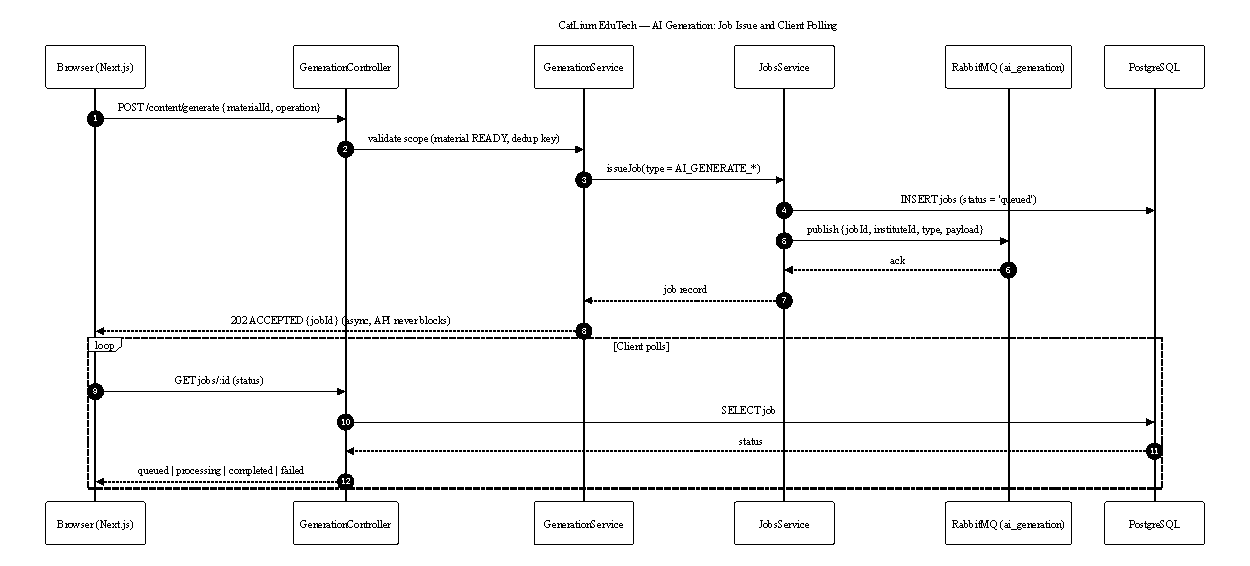
\includegraphics[width=711.5pt]{figures/ai-generation-issue-sequence-bw.pdf}
\caption{Asynchronous AI generation, part 1: job issue and client polling.}
\label{fig:ai-generation}
\end{sidewaysfigure}

\begin{sidewaysfigure}[p]
\centering
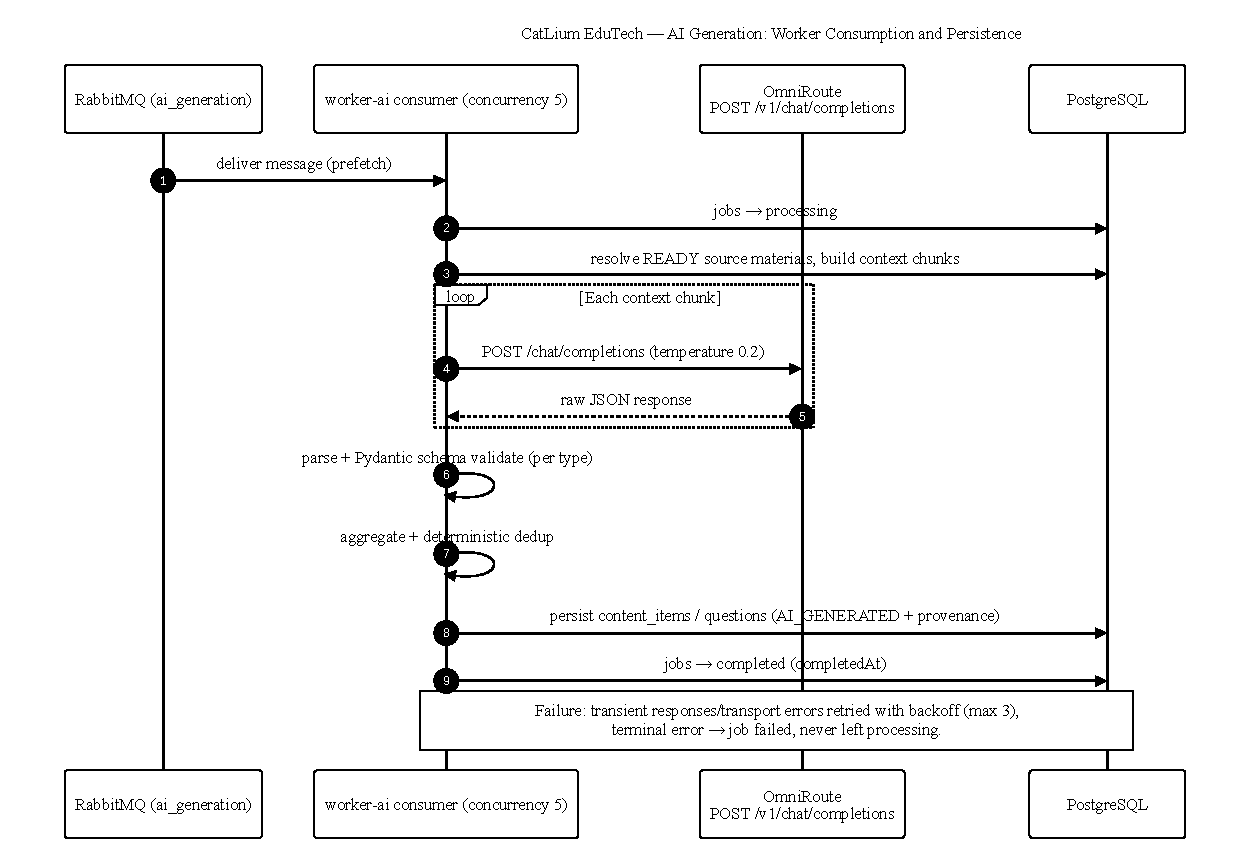
\includegraphics[width=580.4pt]{figures/ai-generation-consume-sequence-bw.pdf}
\caption{Asynchronous AI generation, part 2: worker consumption, OmniRoute
calls, and persistence.}
\label{fig:ai-generation-part2}
\end{sidewaysfigure}

\section{Question Types and the Question Bank}

\sectionmark{Question Bank}
Question types are \emph{data}: the seeded global starters cover
\texttt{MCQ}, TRUE/FALSE, FILL-IN-BLANK, DEFINITION, VERY-SHORT/SHORT/BRIEF/LONG
answer, MATCH-THE-FOLLOWING, CASE-STUDY, and NUMERICAL types, and institutes
may define custom types with their own instructions and defaults. Each type
carries an \texttt{answer\_format} (\texttt{MCQ} | TRUE\_FALSE | FILL\_IN\_BLANK |
TEXT | MATCHING | NUMERICAL) and an objective/subjective kind; the format is
copied onto each question at write time so validation and evaluation always
know the shape of the answer.

The question bank \emph{is} the \texttt{questions} table: stems are scoped to a
subject (optionally chapter/topic), carry difficulty, explanation, an
approval state (\texttt{PENDING} only for staging; new questions are
\texttt{APPROVED}), a source, and provenance. Generation can target a single
type or a full \emph{bank bucket} plan built from question types and a
difficulty distribution (default 34/33/33 across EASY/MEDIUM/HARD), with
per-type minima raised to the type's floor and exact-sum allocation by the
largest-remainder method. Generation is pattern-aware: \texttt{ensurePatternCoverage}
reports COVERED, AWAITING\_APPROVAL, INSUFFICIENT, or GENERATING and queues
exactly the deficit when generating. The worker de-duplicates identical stems
within a batch and inserts questions directly as APPROVED+ACTIVE. Bank
analytics (total/usable, by type, by difficulty) and set management complete
the surface.

\section{Paper Patterns (Blueprints)}

A paper pattern is a blueprint: a title, a subject set
(\texttt{paper\_pattern\_subjects}), a status lifecycle
(\texttt{DRAFT $\rightarrow$ REVIEW $\rightarrow$ APPROVED}), an optional
locked flag, a version, a source type (\texttt{MANUAL}, \texttt{TEXT},
\texttt{MATERIAL}, \texttt{PREVIOUS\_YEAR\_PAPER}), and a structural JSONB that
declares up to 50 sections, each with rules for question type, counts, marks,
compulsoriness, attempt counts, and difficulty/topic distributions. Fields
left \texttt{null} are explicitly \emph{unknown}, never fabricated. Patterns
can be analysed by AI to draft a \texttt{REVIEW} blueprint from a source, and
validated deterministically (the validate endpoint returns
\texttt{\{valid, errors\}}); only \texttt{APPROVED} patterns drive generation
or assessment creation, and approval auto-locks the blueprint. Deterministic
extraction of a pattern from an uploaded source file creates the pattern
immediately and then runs a queued extraction job. Access is staged: DRAFT and
REVIEW are owner-and-admin, APPROVED is pure academic scope.

\section{Question Papers}

A question paper is a fixed snapshot selection of bank questions against a
pattern for student-facing distribution. It stores a scope, instructions,
duration, max marks, and a junction (\texttt{question\_paper\_questions}) that
freezes marks, sections, and sort order at selection time so exports stay
stable. Selection from a pattern replaces the set and re-applies the pattern
rules; coverage computation reports OK, SHORT, EXCESS, or TYPE\_MISMATCH, and
an underserved paper can generate exactly the missing items. A paper converts
to a DRAFT assessment by copying its junction, without re-selection. Papers
may also be produced by deterministic extraction from a source document, with
candidate questions placed in a shared review tray.

\section{Assessments and Attempts}

Assessments are authored resources with a title, scope, timing
(\texttt{starts\_at}/\texttt{ends\_at}), duration, max marks, instructions, and
an explicit state machine \texttt{DRAFT $\rightarrow$ PUBLISHED $\rightarrow$
ACTIVE $\rightarrow$ COMPLETED}, with an unpublish transition DRAFT-ward while
not started. Authoring restricts edits to DRAFT; the publish action re-checks
every link is APPROVED and ACTIVE, that the assessment is scoped and timed, and
that its blueprint coverage is sufficient. Questions can be linked directly or
auto-selected from an approved pattern by type and difficulty. A completed
assessment is terminal.

\subsection{Attempts and evaluation}

An attempt is a timed, snapshot-based student response:
\begin{itemize}
  \item \textbf{Start} is allowed for a published/active assessment within its
  schedule window, with one in-progress attempt per student (enforced by a
  partial unique index and surfaced as \texttt{409}). The full question set is
  snapshotted server-side (stem, type, format, marks, payload); the student
  view is sanitized so answer keys are never sent before answering.
  \item \textbf{Answer saving} validates the answer against its format (for
  example, an MCQ choice id must exist in the choices) and upserts on the
  unique attempt-question pair, guarded by \texttt{FOR UPDATE} on the attempt.
  \item \textbf{Deadline expiry} is enforced server-side: a past-deadline
  in-progress attempt is atomically transitioned to \texttt{EXPIRED} and
  evaluated in the same transaction, so it is never observable as both
  terminal and unevaluated.
  \item \textbf{Evaluation} dispatches on the answer format for the objective
  formats (MCQ, true/false, fill-in-the-blank, matching, numerical). Text and
  custom answers are recorded but never auto-graded (the marker records zero
  marks for them); this keeps the scoring contract honest and defers
  essay-grade automation to the checking-system scope.
  \item \textbf{Submission} is idempotent; the result endpoint reveals
  correctness and awarded marks only for the student's own terminal attempt,
  and the analysis surfaces are aggregate (score distribution, per-question
  accuracy, topic and difficulty performance) with no student-level answer
  data leakage.
\end{itemize}

\section{Practice}

Practice is deliberately ungraded. \texttt{practice\_sessions} run in
\texttt{FLASHCARD} or \texttt{QUESTION} mode: flashcards show card backs from
a content item; question mode presents bank questions. Each session snapshots
its items at start (sanitized), and a per-item response records an
\texttt{AGAIN}/\texttt{GOOD} rating (flashcard) or the answer plus a
correctness flag (question) computed by the same graded dispatcher --- but there
is no score, no ledger, and no analytics. Feedback is instant and per-item:
the answer key is revealed only after the item is answered, in-session. One
open session per source is enforced, and sessions complete idempotently.

\section{Exports}

All export routes share one visual model --- a document of typed blocks
(headings, paragraphs, bullets, steps, flashcards, questions, tables,
formulas, examples, callouts, timelines, diagrams, further-learning lists) ---
from which the PDF, DOCX, and XLSX renderers and the web preview draw. PDF is
produced with real Chromium via a shared lazy browser; DOCX with a document
library; XLSX with a small dependency-free worksheet writer (one worksheet per
table block). Question exports are arranged either by rank order for teacher
sets or by the pattern's section order for pattern-based papers; a
\texttt{paper}/\texttt{answers} flag toggles student-facing (no answers) versus
teacher (answer-key) renderings. Every export/preview route is explicitly
restricted to institute admins and teachers and evaluates academic scope
through the authoritative read gate of the source module, resolving out-of-scope
requests to \texttt{404}.

\section{Asynchronous Job Lifecycle}

All of the above heavy operations ride the generic job subsystem
(\texttt{jobs}): \texttt{queued $\rightarrow$ processing $\rightarrow$
completed | failed | cancelled}, plus a transient \texttt{cancelling} for
in-flight work. Jobs are tenant-scoped, carry their requester for
accountability, and may be retried when failed or cancelled. Coordinator-owned
job types (OCR/enhancement/extraction) are never published to the broker and
are adopted by the sweep; AI and extraction types are reserved to guarded
paths. Publication failures mark the job failed rather than leaving a silent
orphan, and a partial unique index prevents duplicate live generation jobs per
source.
\chapter{Implementation Details}
\label{ch:implementation}

\begin{center}
\textit{This chapter details the implementation: the technology stack, the
repository structure, the NestJS backend, the Python workers, the OCR service,
the web client, and the deployment infrastructure.}
\end{center}

\vspace*{\fill}
\clearpage
\section{Technology Stack}

\noindent Table~\ref{tab:stack} summarises the implemented technology stack.

\begin{table}[htbp]
\centering
\small
\begin{tabular}{@{}p{4.3cm}p{10.2cm}@{}}
\toprule
\textbf{Component} & \textbf{Technology} \\
\midrule
API framework & NestJS (TypeScript, ES2022, NodeNext modules, strict mode) \\
Web client & Next.js (App Router) \\
OCR service & FastAPI (Python 3.12+) \\
Workers & Python 3.12+, pika (direct AMQP consumption) \\
Database & PostgreSQL 17, Drizzle ORM \\
Message broker & RabbitMQ 3 \\
AI integration & Internal OpenAI-compatible gateway (OmniRoute) \\
Validation & Zod (TypeScript), Pydantic (Python) \\
OCR engines & PyMuPDF (embedded text), PaddleOCR (fallback) \\
Deployment & Docker Compose, nginx, Cloudflare Tunnel \\
Build & pnpm workspaces, Turborepo \\
\bottomrule
\end{tabular}
\caption{Implemented technology stack.}
\label{tab:stack}
\end{table}

\section{Repository Structure}

\noindent The monorepo is organised as follows:

\begin{itemize}
  \item \texttt{apps/api} --- the NestJS modular monolith (twenty feature
  modules plus application, database, and health scaffolding);
  \item \texttt{apps/web} --- the Next.js client;
  \item \texttt{apps/ocr} --- the FastAPI OCR service;
  \item \texttt{apps/workers} --- the Python async workers
  (\texttt{worker/} AI and material consumers, \texttt{ocr-worker/} pull
  client);
  \item \texttt{packages/contracts} --- shared API contracts and Zod schemas,
  imported by both web and API;
  \item \texttt{packages/database} --- Drizzle schema, 48 migrations, and the
  database client;
  \item \texttt{packages/auth}, \texttt{packages/ai}, \texttt{packages/shared}
  --- shared authentication, AI, and common utilities;
  \item \texttt{infrastructure/compose} --- the Docker Compose definitions;
  \item \texttt{docs} --- architecture, proposal, status, tracker, and
  user-validation documentation.
\end{itemize}

\noindent TypeScript is compile-strict: ESM with explicit \texttt{.js} import
extensions, no \texttt{any} without an explicit exemption, and a single
\texttt{pnpm typecheck} covering all workspaces. Shared contracts keep the web
client and the API on the same DTOs, while Pydantic models on the Python side
re-validate worker inputs at the boundary.

\section{Backend (NestJS API)}

\noindent Each feature area is a standalone NestJS module
(\texttt{*Module}, \texttt{*Controller}, \texttt{*Service}, \texttt{*DTO}).
Cross-cutting concerns are centralised: the global guard and exception
infrastructure (Chapter~\ref{ch:security}), a DTO validation layer built on
Zod schemas from the contracts package, and Drizzle repositories that always
apply an \texttt{institute\_id} filter. Long-running operations from any
controller call \texttt{JobsService}, which provides the insert-then-publish
job lifecycle, cancellation, retry with deduplication, and status queries.
Routing uses one global prefix \texttt{/api/v1}; the health endpoint lives at
\texttt{GET /api/v1/health}.

\section{AI and Material Workers (Python)}

\noindent The Python workers are plain long-running processes that consume
RabbitMQ queues directly over AMQP (pika), rather than a task framework: the
AI consumer binds \texttt{ai\_generation} with bounded concurrency (default 5)
and prefetch, and the material consumer binds \texttt{jobs}. On start, a
worker recovers stale queued messages so that no work is lost across worker
restarts. Generation work resolves READY source materials from the database,
builds a context budget (a bounded character window divided into overlapping
chunks), calls the model through OmniRoute (\texttt{POST
/v1/chat/completions}), parses and Pydantic-validates each response, then
writes results directly to PostgreSQL with provenance and deterministic
de-duplication. Transient failures and transport errors are retried with
backoff (maximum three attempts); terminal errors settle the job as failed.
The material-enhancement pass runs entirely inside the \emph{API} coordinator
(deterministic, no model), not in a worker.

\section{OCR Service and OCR Worker}

\noindent The OCR service is a dependency-lean FastAPI application with no
business-domain knowledge. It exposes \texttt{GET /health} and extraction
logic that, per page, first attempts PyMuPDF embedded text and falls back to
rasterisation + PaddleOCR when the embedded text is too short; its output is
then passed through a deterministic character-normalization pass. The
standalone \texttt{ocr-worker} package is a pull client: it heartbeats, claims
chunks from the API's worker endpoints, downloads source bytes from the
corresponding read route, runs the extraction range locally, and submits page
results with a page-count field. Legacy one-shot extraction (a file posted to
the OCR service and text returned synchronously into a material) is retained
for compatibility but is not the primary path.

\section{Web Client (Next.js)}

\noindent The web client is built on the App Router and consumes the shared
contracts package. Tenancy is client-side state: the active institute id is
kept in local storage, the API client attaches \texttt{x-institute-id} and the
CSRF header on every request, and a single-flight refresh handles session
renewal with an outcome that never logs the user out on an unavailable
network. UI components are minimal and dependency-light (a small set of
presentational components rather than a component library), and the
institute-switcher shows the resolved institute-domain permissions per
membership so navigation adapts to what the user may do.

\section{Infrastructure and Deployment}

\noindent The single \texttt{docker-compose.yml} defines 12 services:
PostgreSQL~17, Redis~7, RabbitMQ~3, a one-shot migrate runner, the API, the
web client, nginx, the Cloudflare Tunnel sidecar, OmniRoute, the OCR service,
and the two worker images. In the production shape nothing publishes a host
port; a development override binds 127.0.0.1 loopback ports (nginx on
\texttt{8080} by default) for local tooling, and a demo overlay adds seed data
and a worker-to-gateway wiring. Dockerfiles are dependency-first: pnpm
workspace installs run on a shared cache mount so that build layers for
third-party dependencies only rebuild when their manifests change, keeping
whole-stack rebuilds fast while the running containers never hot-reload source
code (this is why every code change to the API, web, or workers requires a
deliberate rebuild and verification step). The nginx configuration splits
paths exactly as described in Chapter~\ref{ch:architecture}; a Cloudflare
Tunnel with one public hostname is the only ingress.
\chapter{Testing and Validation}
\label{ch:testing}

\begin{center}
\textit{This chapter presents the testing and validation of the
implementation: the three-tier testing strategy, the unit and integration
suites, security validation, manual end-to-end validation, and the accepted
limitations of testing.}
\end{center}

\vspace*{\fill}
\clearpage
\section{Testing Strategy}

\noindent The project applies a three-tier test strategy:

\begin{enumerate}
  \item \textbf{Unit tests.} Pure-logic modules (guards, policies, validation,
  parsers, bucket planners, renderers, writers) are tested with
  \texttt{node:test} in the API.
  \item \textbf{Database-gated integration suites.} Flows that touch real
  PostgreSQL (academic scope resolution, authorization regression, session
  hardening, OCR worker flow, export scope, job ownership) run as
  \texttt{*.integration.ts} suites against a test database.
  \item \textbf{Manual and end-to-end validation.} A seeded demo dataset drives
  user-observable flows (login, upload, generation, scheduling, attempts,
  exports), recorded in a standing user-validation log.
\end{enumerate}

\noindent Code standards add a fourth gate: \texttt{pnpm typecheck} (strict
TypeScript across all workspaces) and \texttt{pnpm lint} run on the API, web,
and worker sources, and the Python packages are checked with \texttt{ruff}
and \texttt{mypy} (strict mode) plus pytest suites.

\section{API Unit Tests}

\noindent The API suite currently contains 226 tests across 15 suites, all
passing (verified at the time of writing; a full run reports
\texttt{tests 226, suites 15, pass 226, fail 0}). Coverage concentrates on the
non-trivial, security-relevant logic:

\begin{itemize}
  \item \textbf{Authorization and CSRF.} permission catalogue semantics
  (default-deny, \texttt{manage} implication, role/pass composition),
  double-submit CSRF decisions, and cookie attributes;
  \item \textbf{OCR.} coordinator utilities, page inspection/aggregation, and
  worker registry validation;
  \item \begin{sloppypar}\textbf{Material intelligence.} the deterministic
  enhancer (block classification, keep/exclude/review findings, segment
  mapping);\end{sloppypar}
  \item \textbf{Word and worksheet generation.} DOCX and XLSX renderers, PDF
  smoke tests, question/paper document builders;
  \item \textbf{Question planning.} batch bucket building (difficulty
  distribution allocations that sum exactly), batch planning floors/ceilings,
  paper-pattern demand and validation, and the deterministic extractor;
  \item \textbf{Scope resolution and identity.} scope-chain resolution and
  login origin checks.
\end{itemize}

\section{Integration Suites}

\noindent Eleven database-backed integration suites exercise cross-service
behaviour that unit tests cannot:

\begin{itemize}
  \item \texttt{identity/auth-session.integration.ts} --- F1--F5 session
  hardening: session-bound access tokens, strict one-time rotation,
  lineage revocation, logout/revoke semantics, user-status gating, non-
  enumerating login, and password-reset one-shot flow (14 tests);
  \item \texttt{authorization/authz-regression.integration.ts} --- the guard
  chain end to end;
  \item \texttt{\seqsplit{authorization/academic-scope.integration.ts}} and
  \texttt{\seqsplit{resource-scope.integration.ts}} --- scope resolution for teachers and
  students and the 404/403 contract;
  \item \texttt{\seqsplit{authorization/mod-3-export-scope}} /
  \texttt{\seqsplit{mod-4-attempts-scope}}
  and \texttt{\seqsplit{phase-m-remediation.integration.ts}} --- the remediation fixes of
  the Phase~M security audit stay fixed;
  \item \texttt{\seqsplit{authorization/job-ownership.integration.ts}} --- job requester
  stamping and cross-institute adoption defence;
  \item \texttt{academic-structure/*.integration.ts} --- teacher assignments
  and student placements;
  \item \texttt{ocr/ocr-worker-flow.integration.ts} --- the coordinator +
  claim + lease + finalize loop against a real database.
\end{itemize}

\section{Security Validation}

\noindent Security behaviour was validated in a dedicated audit phase that
compared the implementation against a written threat model. It found and
remediated: a HIGH-severity export path that could expose answer keys to
unauthorized teachers (now every export route carries an explicit role
restriction and resolves scope through the authoritative module gate); a
MEDIUM-severity path by which a job created in one institute could be adopted
with another institute's process; and two LOW-severity issues (jobs now record
their requester; stale institute context is cleaned on logout and on
unauthorized responses). Regression suites in the repository keep these fixes
verified.

\section{Manual and End-to-End Validation}

\noindent A seeded demo workload (institutes, academic structure, materials,
syllabi, generated content and questions, patterns, assessments, attempts, and
practice sessions) is exercised through the web client and recorded in the
user-validation log, covering the primary journeys that unit and integration
suites cannot reach: multi-institute sign-in and switching, chunked uploads
through the browser, OCR progress and corrections, AI-generation status
polling, assessment scheduling and timing, attempt submission and the result
view, practice sessions, and printed exports.

\section{Limitations of Testing}

\noindent Browser-level end-to-end automation is not yet present; web
journeys are validated manually against the seeded dataset. OCR accuracy and
AI output quality are validated functionally (structure, schema conformance,
provenance) rather than by quantitative metrics; the AI pipeline's
de-duplication and schema-validation guarantees are covered by worker
unit tests in the Python packages.
\chapter{Results and Discussion}
\label{ch:results}

\section{Delivered Capabilities}

\noindent Table~\ref{tab:results} maps the objectives of
Chapter~\ref{ch:introduction} to the delivered, verified capabilities.

\begin{table}[h]
\centering
\small
\begin{tabular}{@{}p{2.9cm}p{11.4cm}@{}}
\toprule
\textbf{Objective} & \textbf{Delivered capability} \\
\midrule
Tenancy and identity & Multi-institute deployment with memberships, roles,
and a permission catalogue; every query tenant-scoped by the enforcement
layers. \\
Academic structure & Years, classes, divisions, subjects, chapters, topics,
offerings, teacher assignments, student placements/enrollments; academic scope
derived from current DB state. \\
Materials and OCR & Chunked upload; distributed OCR (embedded-text-first,
PaddleOCR fallback); page corrections; coordinator-owned chunk leasing. \\
Syllabus intelligence & AI analysis into per-subject structure and context
with PROPOSED$\rightarrow$CONFIRMED lifecycle and per-subject versioning. \\
Aided content creation & Typed, versioned content items generated from
eligible sources with provenance and in-place regeneration. \\
Question assets & Data-driven question types (11 global seeds), an approved
question bank, pattern-aware generation, paper patterns, and question papers. \\
Examination & Blueprint-driven assessments with schedule validation,
snapshot attempts, server-side objective evaluation, and aggregate analytics. \\
Practice & Ungraded flashcard and question sessions with instant per-item
feedback. \\
Export & Single-model PDF (Chromium), DOCX, XLSX rendering for content,
questions, papers, patterns, and results; preview equals export. \\
Security & Session-bound tokens, strict rotation with lineage revocation,
double-submit CSRF, DB-fresh authorisation, academic scope, and a
documentation-verified audit with no open high findings. \\
\bottomrule
\end{tabular}
\caption{Objectives versus delivered capabilities.}
\label{tab:results}
\end{table}

\section{Validation Summary}

\noindent The implementation is supported by 226 passing API unit tests,
eleven database-backed integration suites, strict type-checking and linting
across TypeScript and Python, a standing user-validation log driven by a
seeded demo dataset, and a security audit whose findings are all remediated
and covered by regression tests.

\section{Discussion}

\noindent Three architectural choices deserve discussion.

\subsection{Modular monolith over microservices}

Keeping the business modules in one deployable unit means authorization
evaluation, tenancy scoping, and database transactions stay simple and local.
The two genuinely independent workloads --- OCR and AI generation --- were
pushed out of the monolith to dedicated components behind queues, which is
where elasticity actually matters. This matches the project's standing
decision to avoid premature microservices.

\subsection{Permission + scope instead of pure RBAC}

Nesting academic scope under the permission model closes the classic RBAC
leak: a teacher with \texttt{questions.update} still cannot touch a question in
a subject they do not teach, because the scope gate evaluates the resource's
subject against the teacher's assignment-derived subject set. The cost is a
per-query scope predicate, which is cheap relative to the guarantee it gives.
The 404-for-reads / 403-for-writes asymmetry keeps resource existence hidden
from unauthorized actors.

\subsection{Coordinator-owned OCR versus queue-based work}

OCR workers are heterogenous and expected to be occasionally offline, so chunk
ownership is expressed as a \emph{lease} with heartbeat renewal and
sweep-based reclamation rather than an unbounded queue message. This design was
chosen over retried queue delivery and validated against a real database in
the OCR integration suite. A side effect is that the OCR pipeline can be
incrementally scaled by adding workers with no coordinator downtime.

\section{Limitations}

\noindent The following limitations are accepted and documented in the
repository:

\begin{itemize}
  \item \textbf{Selection randomness.} Pattern-to-paper selection is
  deterministic; randomization within a bucket is not implemented.
  \item \textbf{Question-paper immutability.} The question-paper junction
  keeps a live foreign key to the bank question; a later edit to that question
  can leak into paper exports (attempts, by contrast, are true snapshots).
  \item \textbf{Provenance reads.} The \texttt{source\_pattern\_id} column is
  write-only; there is no read path exposing a question's origin pattern in the
  API or web client.
  \item \textbf{Attempt-N-of-M.} Attempt numbering and max-attempt limits are
  presentation metadata only; all linked questions are always evaluated.
  \item \textbf{Duplication detection.} Within-batch exact-stem de-duplication
  and a prompt instruction are used; there is no similarity/embedding scan
  across the bank.
  \item \textbf{Scope granularity.} Academic scope is currently subject-set
  based; the designed offering-level scope (\texttt{offeringId} column) is
  not yet in the schema.
  \item \textbf{Rate limiting.} The global throttle is in-memory per instance;
  a distributed (Redis-backed) limiter is deferred until cross-instance
  rate limiting is needed.
  \item \textbf{OCR/AI quality metrics.} Extraction accuracy and generated
  content are validated structurally; quantitative quality metrics are not
  produced.
\end{itemize}

Further deferred scope --- online answer sheets (FORM), OMR, on-screen
marking, automated text grading, CRUD for a full \texttt{SUPER\_ADMIN}
institute lifecycle UI, and web-level end-to-end automation --- is documented
in Chapter~\ref{ch:conclusion}.
\chapter{Conclusion and Future Scope}
\label{ch:conclusion}

\begin{center}
\textit{This chapter concludes the project and lists the identified future
scope together with the extensions that the architecture is structured to
support.}
\end{center}

\vspace*{\fill}
\clearpage
\section{Conclusion}

\noindent This project set out to build a single, tenant-isolated platform that
walks a college through its content-preparation and examination lifecycle, and
it delivered one: institutes are provisioned with users, roles, and
permissions; academic structure is modelled and turned into enforceable
academic scope; uploaded materials are OCR-processed by distributed workers
into reusable text; syllabus documents are analysed into confirmed
curricula; study content and question banks are generated with provenance
through an internal AI gateway; paper patterns, question papers, and
scheduled assessments are authored, published, attempted, and evaluated
server-side for objective answer formats; aggregate analytics follow; an
ungraded practice mode supports revision; and content, papers, patterns, and
results export to PDF, DOCX, and XLSX.

The engineering outcome is equally deliberate. The system is a modular
monolith with asynchronous workers, a single PostgreSQL database, strict
tenant scoping at the enforcement layers, and a security design ---
session-bound tokens, strict refresh rotation, double-submit CSRF, DB-fresh
permission evaluation from an explicit 83-key catalogue, academic scope, and a
documentation-verified audit --- that resists the access-control leaks that
plague role-name-based systems. The implementation is validated by 226
passing unit tests, eleven database-integrated suites, strict type-checking
and linting across both languages, and a recorded user-validation pass, with
no unresolved security findings.

\section{Future Scope}

\noindent The following extensions are identified and left for future work:

\begin{enumerate}
  \item \textbf{Checking-system features} --- online answer sheets (FORM),
  OMR scanning, and on-screen marking, including automated grading of
  subjective text answers, which the current evaluation contract deliberately
  records but does not grade.
  \item \textbf{Attempt mechanics} --- true per-attempt N-of-M numbering with
  maximum-attempt enforcement and auto-replenishment after selection.
  \item \textbf{Offering-level academic scope} --- introducing the designed
  \texttt{offeringId} binding so resources can additionally be restricted to a
  single class--subject offering.
  \item \textbf{Selection and deduplication quality} --- randomized selection
  within pattern buckets, similarity-based de-duplication across the bank, and
  a read path for question origin patterns.
  \item \textbf{Platform administration surface} --- a working
  \texttt{SUPER\_ADMIN} console for institute lifecycle and the OCR worker
  registry.
  \item \textbf{Operational hardening} --- distributed Redis-backed rate
  limiting, S3-backed storage behind the existing storage abstraction,
  quantitative OCR/AI quality metrics, worker observability, and web-level
  end-to-end test automation.
  \item \textbf{Academic export redesign} --- per-topic and per-resource
  exports with richer document formats.
\end{enumerate}

\noindent The architecture is structured so that each extension lands as a new
module or a role-gated surface without disturbing the tenant-isolation and
authorization guarantees that this report describes.

\backmatter
\cleardoublepage
\addcontentsline{toc}{chapter}{References}
\bibliographystyle{IEEEtran}
\bibliography{references}

\chapter*{Glossary}
\addcontentsline{toc}{chapter}{Glossary}

\begin{longtable}{@{}p{4.2cm}p{\dimexpr\textwidth-4.2cm-12pt\relax}@{}}
\toprule
\textbf{Term} & \textbf{Definition} \\
\midrule
\endhead
Assessment & A scheduled examination built from a question paper or question
set, with a start/end period and attempt rules. \\
Attempt & A student's snapshot of an assessment's question set, taken at
start time and later submitted and evaluated. \\
Chapter & A unit of academic structure within a subject, holding topics. \\
Institute & The tenant anchor in the multi-tenant model; all data is scoped
to an institute. \\
Job & An asynchronous unit of work executed by a worker and tracked in the
API with a lifecycle of queued, processing, completed, failed, or cancelled.
\\
Material & An uploaded or text study document processed through the OCR
pipeline. \\
Material Intelligence & The deterministic engine that cleans, structures,
and segments extracted text and maps it to syllabus entities. \\
Membership & The user--institute relationship that carries roles and
determines tenancy. \\
Modular monolith & A single deployable application with clearly bounded
modules, avoiding premature microservices. \\
Multi-tenant & Serving many institutes from one deployment while isolating
their data. \\
OCR & Optical character recognition; conversion of scanned documents and
images into machine-readable text. \\
Paper pattern & A nested structure of sections and question types with
attempt rules that an examination paper must follow. \\
Practice & Ungraded, per-item study sessions of flashcards and questions
with instant feedback. \\
Question bank & The data-driven repository of questions with types,
difficulties, and review status. \\
Question paper & A set of questions assembled against a paper pattern,
exportable to document formats. \\
Role & A permission level granted through a membership: institute
administrator, teacher, or student. \\
Syllabus & The academic subject structure proposed by AI and confirmed by a
teacher. \\
Tenant & An institute whose data is isolated from other institutes in the
same deployment. \\
Vertical slice & A thin end-to-end path through the full system, developed
as the unit of a milestone. \\
\bottomrule
\end{longtable}

\cleardoublepage
\makeatletter\@mainmattertrue\makeatother
\appendix
\chapter{The Permission Catalogue}
\label{app:permissions}

\begin{center}
\textit{This appendix reproduces the full institute-domain and platform-domain
permission catalogue implemented by the authorization module.}
\end{center}

\vspace*{\fill}
\clearpage
\noindent The authorization catalogue is a typed map in code, mirrored into
the \texttt{permissions} table on every API boot and verified for consistency.
Keys are explicit \texttt{resource.action} strings; \texttt{manage} implies
every other action of the same resource. Tables~\ref{tab:perm-institute} and
\ref{tab:perm-platform} reproduce the catalogue.

\begin{table}[htbp]
\centering
\small
\begin{tabular}{@{}p{3.7cm}p{7.7cm}p{2.3cm}@{}}
\toprule
\textbf{Resource} & \textbf{Actions} & \textbf{Keys} \\
\midrule
\texttt{subjects} & read, create, update, delete, manage & 5 \\
\texttt{chapters} & read, create, update, delete, manage & 5 \\
\texttt{topics} & read, create, update, delete, manage & 5 \\
\texttt{content} & read, create, update, delete, manage & 5 \\
\texttt{materials} & read, create, update, delete, manage & 5 \\
\texttt{syllabus} & read, create, update, delete, manage & 5 \\
\texttt{questions} & read, create, update, delete, manage & 5 \\
\texttt{question-types} & read, manage & 2 \\
\texttt{paper-patterns} & read, create, update, delete, manage & 5 \\
\texttt{question-papers} & read, create, update, delete, manage & 5 \\
\texttt{assessments} & read, create, update, delete, manage & 5 \\
\texttt{attempts} & read, create, update, manage & 4 \\
\texttt{practice} & read, create, update, manage & 4 \\
\texttt{exports} & read, manage & 2 \\
\texttt{jobs} & read, update, manage & 3 \\
\texttt{users} & read, create, update, manage & 4 \\
\texttt{roles} & read, create, update, delete, manage & 5 \\
\midrule
\multicolumn{2}{r}{\textbf{Institute domain total}} & \textbf{74} \\
\bottomrule
\end{tabular}
\caption{Institute-domain permission catalogue.}
\label{tab:perm-institute}
\end{table}

\begin{table}[htbp]
\centering
\small
\begin{tabular}{@{}p{3.7cm}p{7.7cm}p{2.3cm}@{}}
\toprule
\textbf{Resource} & \textbf{Actions} & \textbf{Keys} \\
\midrule
\texttt{institutes} & read, create, update, delete, manage & 5 \\
\texttt{ocr-workers} & read, create, update, manage & 4 \\
\midrule
\multicolumn{2}{r}{\textbf{Platform domain total}} & \textbf{9} \\
\bottomrule
\end{tabular}
\caption{Platform-domain permission catalogue.}
\label{tab:perm-platform}
\end{table}

\noindent The catalogue enforces explicit-only semantics: there are no
wildcards, unknown keys resolve to \texttt{false}, and system roles are
seeded from \texttt{BUILT\_IN\_ROLE\_DEFINITIONS} on boot.
\chapter{Application Screenshot Plates}
\label{app:screenshots}

\begin{center}
\textit{This appendix reproduces the colour captures of the running platform,
assembled four-per-page so that the batch occupies as few pages as possible.
All text is black; all UI fills are in colour.}
\end{center}

\vspace*{\fill}
\clearpage

\noindent The plates below were captured against the live deployment
(\texttt{edutech.catlium.in}) through an authenticated teacher workspace
session to demonstrate the feature set actually exercised in this report:
dashboard, subjects, materials, learning content, question bank, question
papers, paper patterns, and assessments.

\begin{figure}[p]
\centering
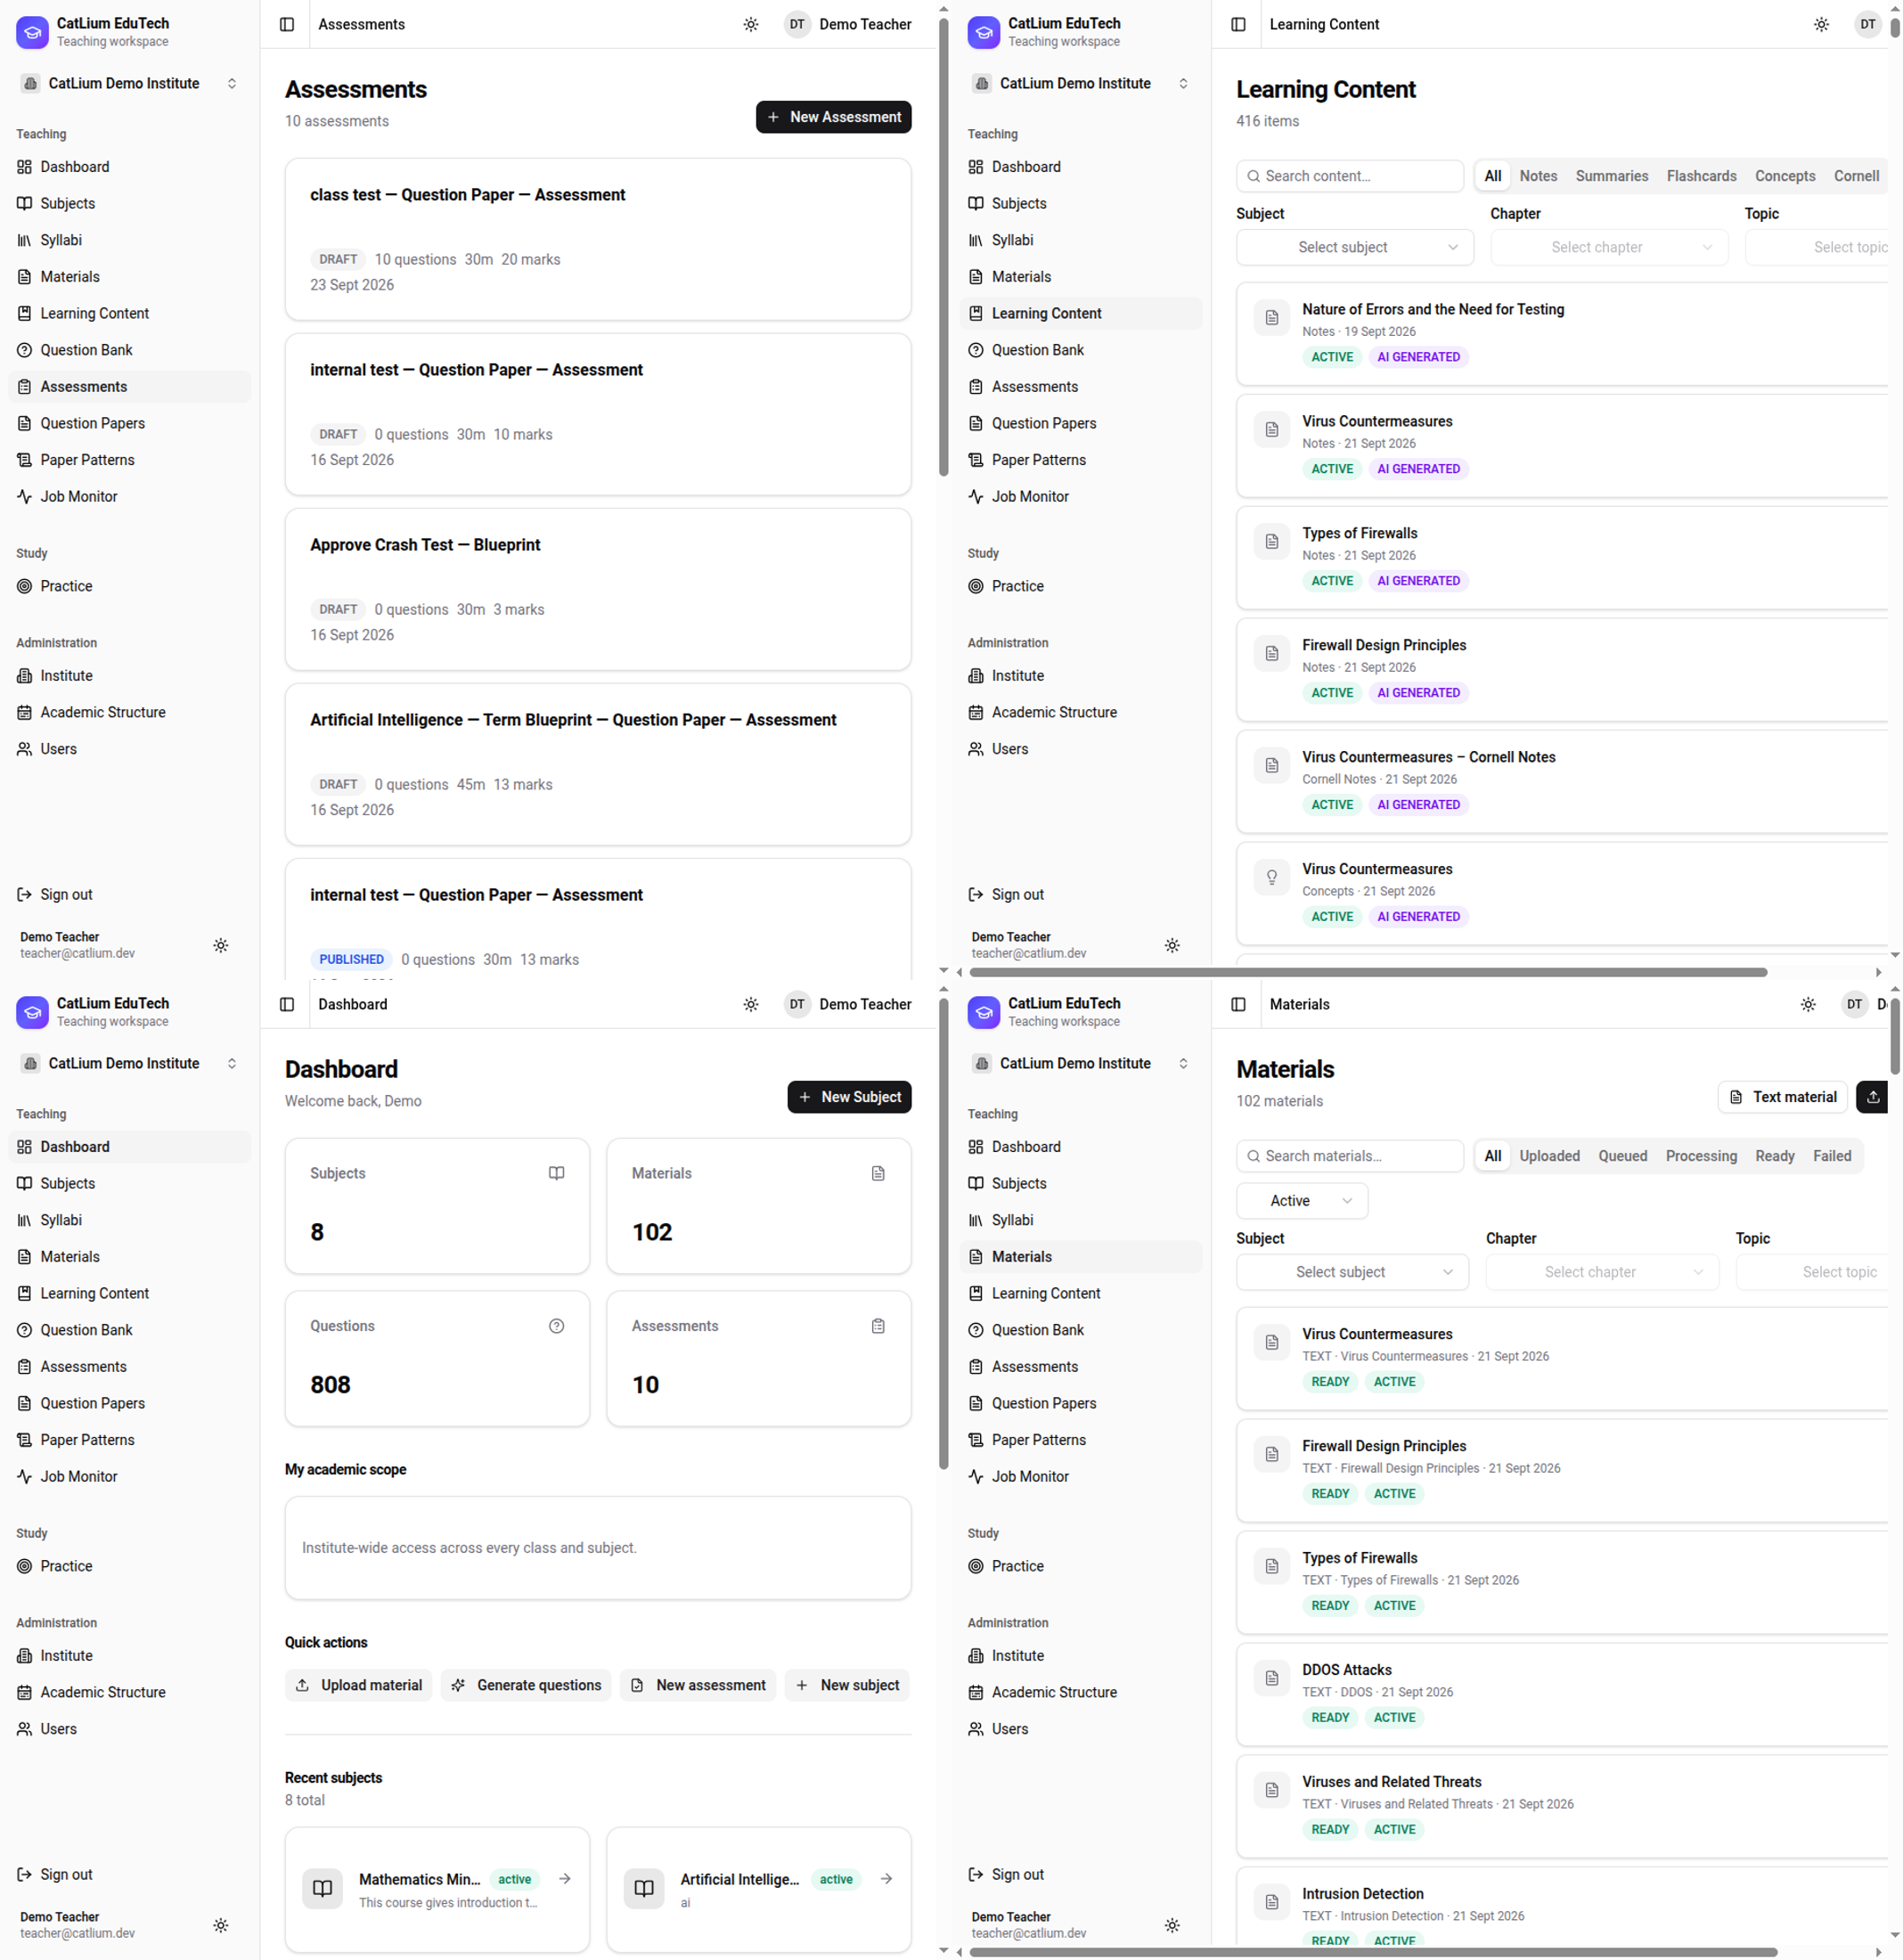
\includegraphics[width=\textwidth,height=\textheight,keepaspectratio]{figures/plate-1.png}
\caption{Plate 1 --- teacher workspace: dashboard, subjects, materials, and
learning content (colour; four per page).}
\label{fig:plate-screenshots-1}
\end{figure}

\begin{figure}[p]
\centering
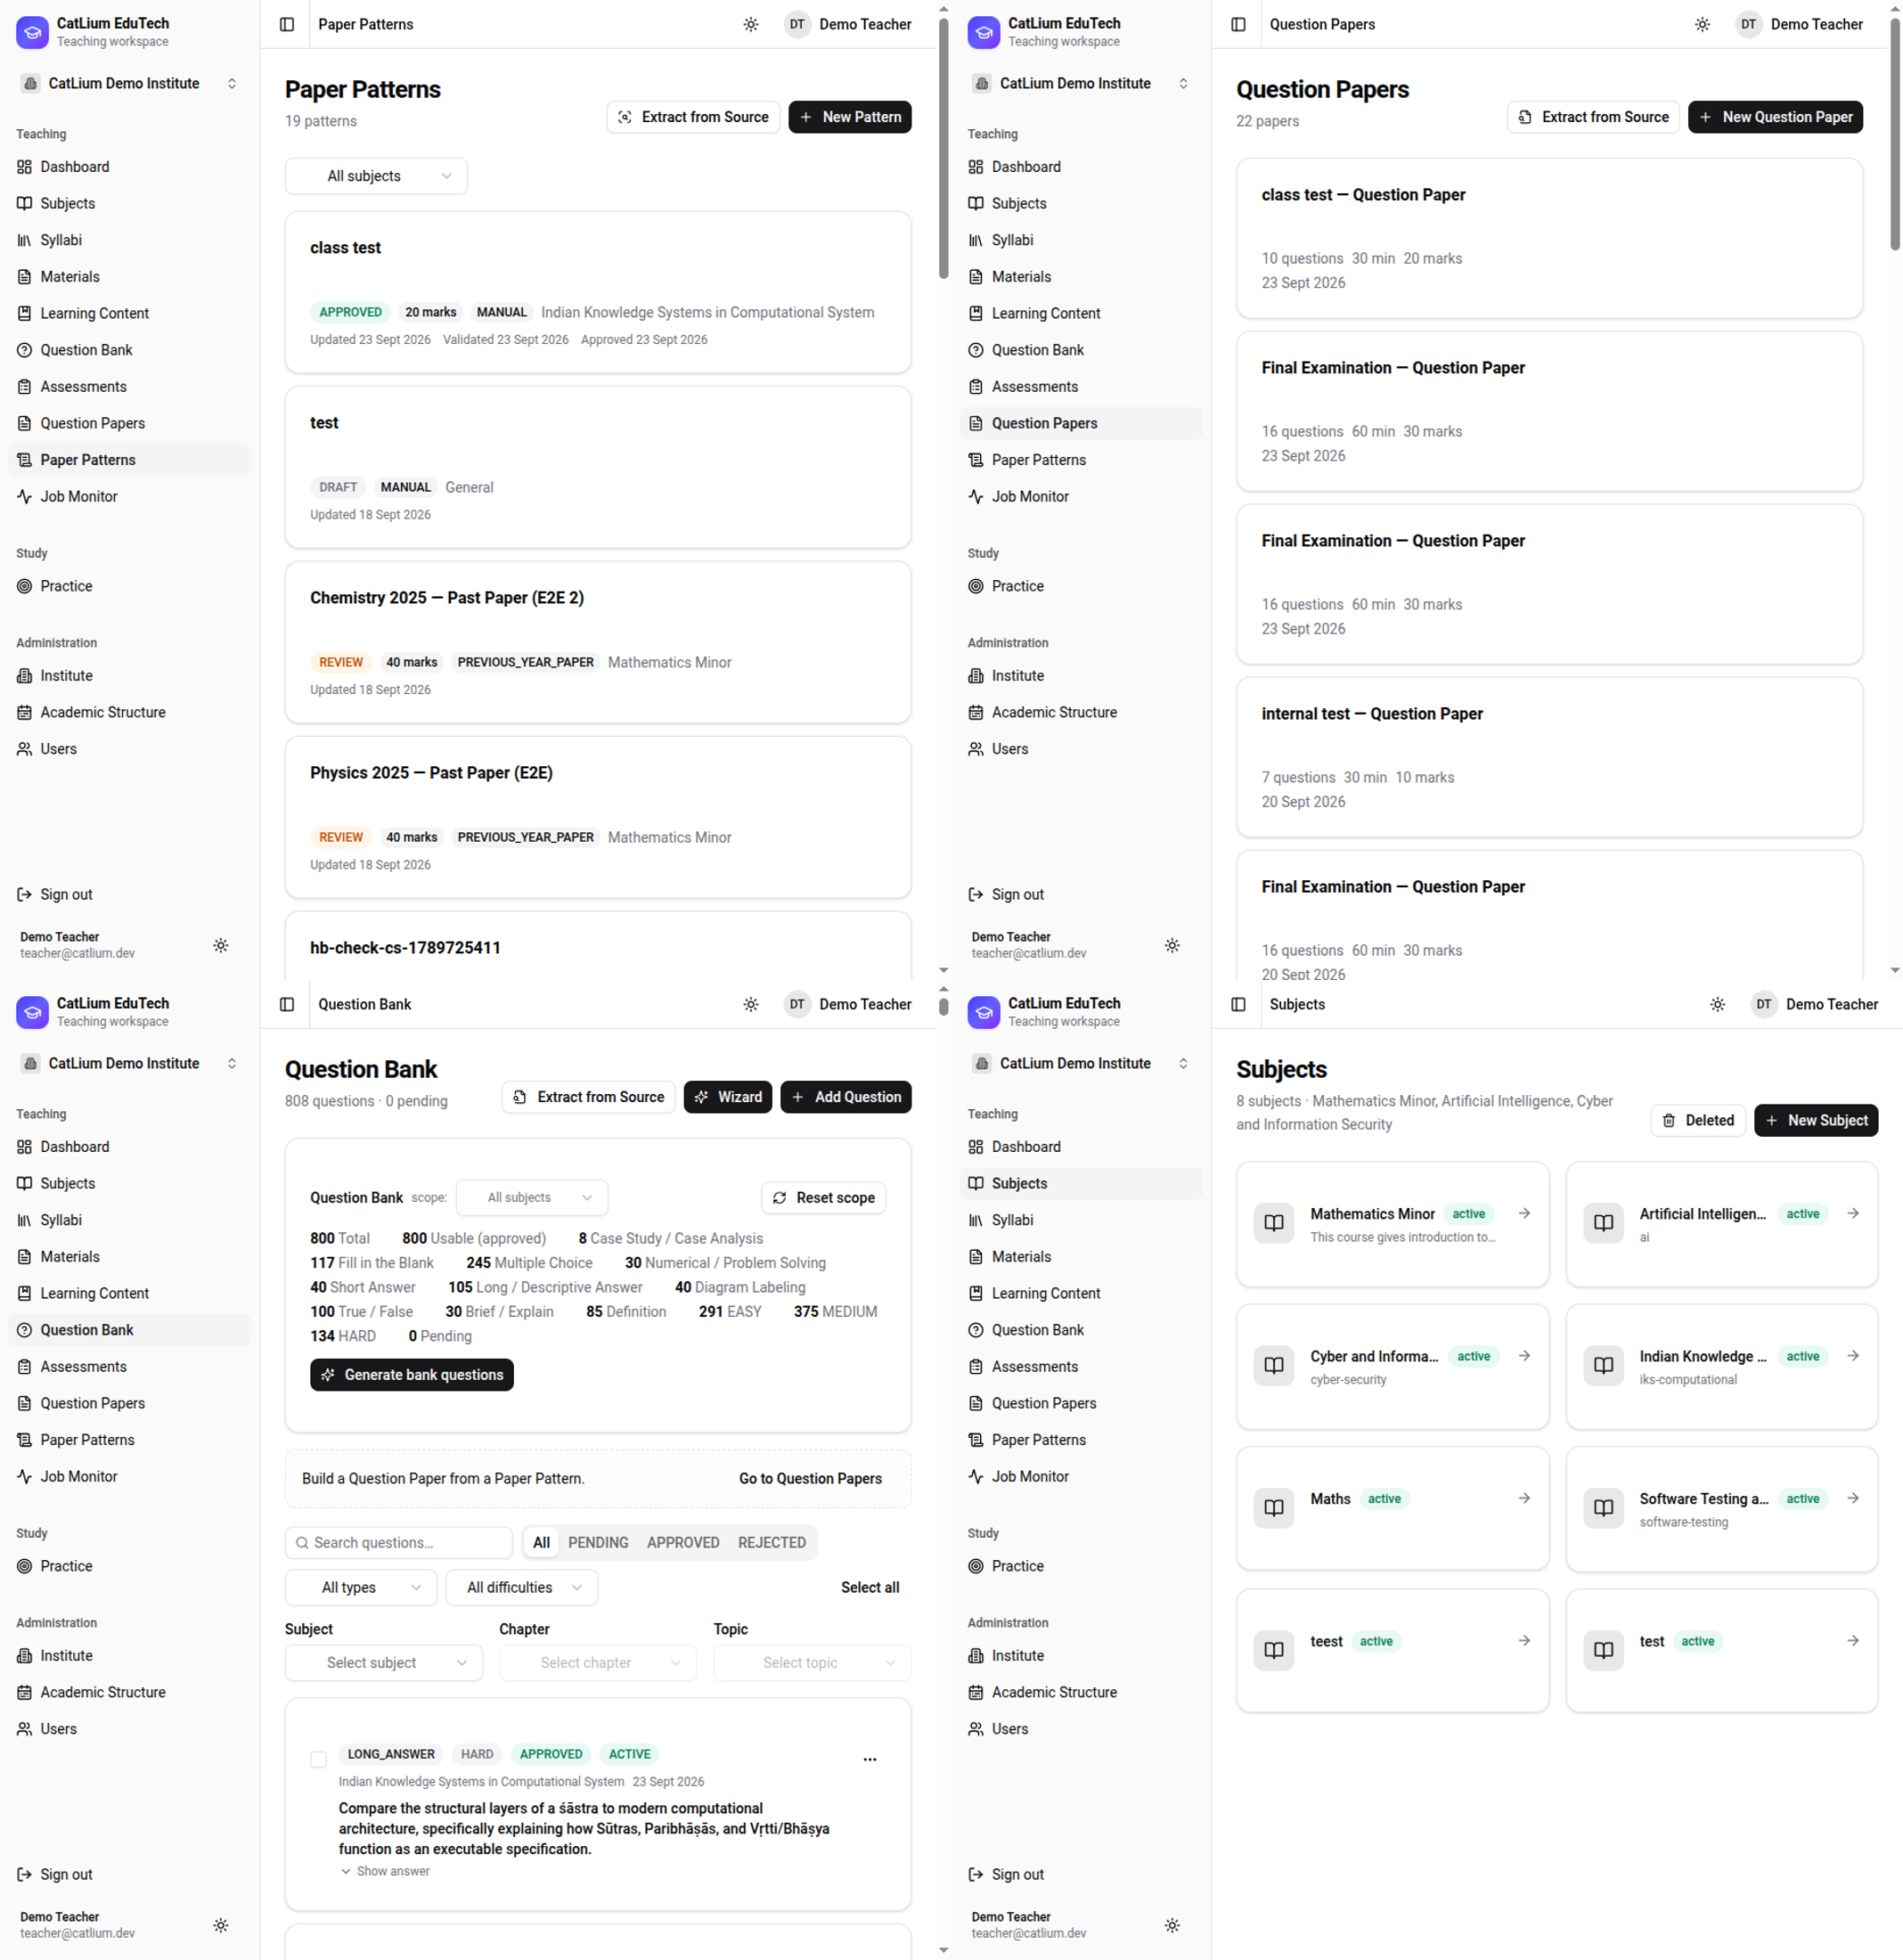
\includegraphics[width=\textwidth,height=\textheight,keepaspectratio]{figures/plate-2.png}
\caption{Plate 2 --- teacher workspace: question bank, question papers, paper
patterns, and assessments (colour; four per page).}
\label{fig:plate-screenshots-2}
\end{figure}

\chapter{Core Environment Variables}
\label{app:environment}

\begin{center}
\textit{This appendix lists the core environment variables that control the
runtime behaviour described in this report.}
\end{center}

\vspace*{\fill}
\clearpage
\noindent Table~\ref{tab:env} lists the configuration variables that most
directly control the runtime behaviour described in this report. All
configuration is via environment variables; the template lives at
\texttt{.env.example} and \texttt{.env} files are never committed.

\begin{table}[htbp]
\centering
\small
\begin{tabular}{@{}p{6.2cm}p{8cm}@{}}
\toprule
\textbf{Variable} & \textbf{Purpose (default)} \\
\midrule
\texttt{JWT\_SECRET} & HS256 signing secret; boot failure in production if
missing. \\
\texttt{ACCESS\_TOKEN\_EXPIRY\_MINUTES} & Access-token lifetime (15). \\
\texttt{REFRESH\_TOKEN\_EXPIRY\_DAYS} & Refresh-token lifetime, sliding (30). \\
\texttt{COOKIE\_SAMESITE} / \texttt{COOKIE\_SECURE} & Cookie posture
(\texttt{lax} / false). \\
\texttt{RATE\_LIMIT\_LIMIT} / \texttt{RATE\_LIMIT\_TTL\_MS} & Global
throttle (100 / 60000). \\
\texttt{AUTH\_RATE\_LIMIT\_LIMIT} / \texttt{AUTH\_RATE\_LIMIT\_TTL\_MS} &
Auth-route throttle (5 / 60000). \\
\texttt{DATABASE\_URL} & PostgreSQL connection string. \\
\texttt{REDIS\_URL} / \texttt{RABBITMQ\_URL} & Cache and broker addresses. \\
\texttt{STORAGE\_LOCAL\_DIR} & Local file-storage root (abstraction for S3). \\
\texttt{INTERNAL\_API\_KEY} & Shared internal-auth header key. \\
\texttt{WORKER\_OCR\_CHUNK\_SIZE} & OCR chunk page count (10). \\
\texttt{WORKER\_OCR\_LEASE\_SECONDS} & Chunk lease duration (300). \\
\texttt{WORKER\_SWEEP\_INTERVAL\_MS} & Coordinator sweep interval (15000). \\
\texttt{WORKER\_AI\_PROVIDER\_URL} & OmniRoute OpenAI-compatible base URL. \\
\texttt{WORKER\_AI\_API\_KEY} & Endpoint key for the AI gateway. \\
\texttt{WORKER\_AI\_MODEL} & Model selection (\texttt{auto}). \\
\texttt{WORKER\_AI\_CONCURRENCY} & Parallel AI job threads (5). \\
\texttt{WORKER\_AI\_MAX\_CONTEXT\_CHARS} & Source context budget per job (40000). \\
\texttt{WORKER\_AI\_CHUNK\_SIZE\_CHARS} & Per-call context chunk (12000). \\
\texttt{WORKER\_AI\_CHUNK\_OVERLAP\_CHARS} & Chunk overlap (400). \\
\texttt{WORKER\_AI\_MAX\_RETRIES} & Transient-failure retry limit (3). \\
\texttt{WORKER\_OCR\_SERVER\_URL} / \texttt{WORKER\_OCR\_WORKER\_ID} /
\texttt{WORKER\_OCR\_API\_KEY} & Standalone OCR worker bootstrap. \\
\texttt{TUNNEL\_TOKEN} & Cloudflare Tunnel credentials (only public ingress). \\
\bottomrule
\end{tabular}
\caption{Core environment variables.}
\label{tab:env}
\end{table}

\end{document}